\chapter{Utilisation avancée des graphes}
\label{chap-advanced-grammars}
\section{Les types de graphes}
\index{Graphe!types de}\index{Types de graphes}
Unitex peut manipuler plusieurs types de graphes qui correspondent aux utilisations
suivantes : flexion automatique de dictionnaires, prétraitement des textes, normalisation
des automates de textes, graphes dictionnaires, recherche de motifs, levée d’ambiguïtés et
génération automatique de graphes. Ces différents types de graphes ne sont pas interprétés
de la même façon par Unitex. Certaines choses comme les sorties sont permises pour certains
types et interdites pour d’autres. De plus, les symboles spéciaux ne sont pas les mêmes en
fonction du type de graphe. Cette section présente donc chacun des types de graphes en
détaillant leurs particularités.


\subsection{Graphes de flexion}
\index{Transducteur!de flexion}\index{Flexion automatique}\index{Graphe!de flexion}
Un graphe de flexion décrit les variations morphologiques associées à une classe de
mots, en associant à chaque variante des codes flexionnels. Les chemins d’un tel graphe décrivent
les modifications à appliquer aux formes canoniques tandis que les sorties contiennent
les informations flexionnelles qui seront produites.


\bigskip
\begin{figure}[!ht]
\begin{center}
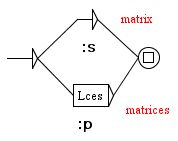
\includegraphics[width=4.5cm]{resources/img/fig6-1.png}
\caption{Exemple de grammaire de flexion}
\end{center}
\end{figure}

\index{Opérateur!\verbc{L}}
\index{Opérateur!\verbc{R}}
\index{Opérateur!\verbc{C}}
\index{Opérateur!\verbc{D}}
\index{Opérateur!\verbc{U}}
\index{Opérateur!\verbc{P}}
\index{Opérateur!\verbc{W}}
\index{\verbc{L}}
\index{\verbc{R}}
\index{\verbc{C}}
\index{\verbc{D}}
\index{\verbc{U}}
\index{\verbc{P}}
\index{\verbc{W}}
\noindent Les chemins peuvent contenir des opérateurs et des lettres. Les opérateurs possibles
sont représentés par les caractères \verb+L+, \verb+R+, \verb+C+, \verb+D+, \verb+U+, \verb+P+ et
\verb+W+.
Les lettres qui ne sont pas des opérateurs sont des caractères. Le seul symbole spécial autorisé est
le mot vide \verb+<E>+.\index{\verbc{<E>}} Il n’est pas possible de faire référence aux dictionnaires
dans un graphe de flexion. Il est cependant possible de
faire appel à des sous-graphes.

\bigskip
\noindent Les sorties sont concaténées pour produire une chaîne de caractères. Cette chaîne est
ensuite concaténée à la ligne de dictionnaire produite. Les sorties à variables n’ont pas de
sens dans un graphe de flexion.


\bigskip
\noindent Le contenu d’un graphe de flexion est manipulé sans aucune variante de casse: les lettres
minuscules restent minuscules, idem pour les majuscules. En outre, la liaison de deux boîtes
est strictement équivalente à la concaténation de leurs contenus munie de la concaténation
de leurs sorties (voir figure~\ref{fig-equivalent-inflection-paths}).\index{Respect!des
minuscules/majuscules}

\bigskip
\begin{figure}[!ht]
\begin{center}
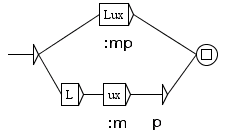
\includegraphics[width=5.5cm]{resources/img/fig6-2.png}
\caption{Deux chemins équivalents dans une grammaire de flexion\label{fig-equivalent-inflection-paths}}
\end{center}
\end{figure}

\bigskip
\noindent Les graphes de flexion doivent être compilés avant de pouvoir être utilisés par le pro-
gramme de flexion.


\bigskip
\noindent Pour plus de détails, voir section
\ref{section-automatic-inflection}.

\subsection{Graphes de prétraitement}
\index{Texte!prétraitement}\index{Grammaires!pour la reconnaissance de fin de phrase}
\index{Grammaires!normalisation!de formes non ambiguës}
Les graphes de prétraitement sont destinés à être appliqués aux textes avant que ceux-ci soient
découpés en unités lexicales. Ces graphes peuvent être utilisés pour insérer ou
remplacer des séquences dans les textes. Les deux utilisations usuelles de ces graphes sont
la normalisation de formes non ambiguës et le découpage en phrases.


\bigskip
\noindent L’interprétation de ces graphes dans Unitex est très proche de celle des graphes
syntaxiques utilisés pour la recherche de motifs. Les différences sont les suivantes:

\begin{itemize}
  \item on peut utiliser le symbole spécial \verb+<^>+ qui reconnaît un retour à la
  	  ligne;\index{\verbc{<^>}}
  \item si l'on travaille en mode caractère par caractère, il est possible d'utiliser 
  	  le symbole spécial \verb+<L>+ qui reconnaît une lettre, telle que définie dans le fichier
  	  alphabet;\index{\verbc{<L>}}
  \item il est impossible de faire référence aux dictionnaires;
  \item il est impossible d’utiliser les filtres morphologiques;
  \item il est impossible d’utiliser le mode morphologique;
  \item il est impossible d’utiliser des contextes.
\end{itemize}

Les figures~\ref{fig-example-sentence-splitting} (page \pageref{fig-example-sentence-splitting})
et~\ref{fig-normalization-grammar} (page \pageref{fig-normalization-grammar}) montrent des exemples
de graphes de prétraitement.


\subsection{Graphes de normalisation de l’automate du texte}
\label{section-normalizing-text-automataon}
\index{Automate!du texte}\index{Texte!automate du!normalisation}
\index{Grammaires!normalisation!de l'automate du texte}
\index{Normalisation!de l'automate du texte}
\index{Normalisation!de formes ambiguës}
Les graphes de normalisation de l’automate du texte permettent de normaliser des formes
ambiguës. En effet, ils peuvent décrire plusieurs étiquettes pour une même forme. Ces étiquettes
sont ensuite insérées dans l’automate du texte, explicitant ainsi les ambiguïtés. La
figure~\ref{fig-tfst-normalization-grammar} montre un extrait du graphe de normalisation utilisé
pour le français.

\bigskip
\begin{figure}[!ht]
\begin{center}
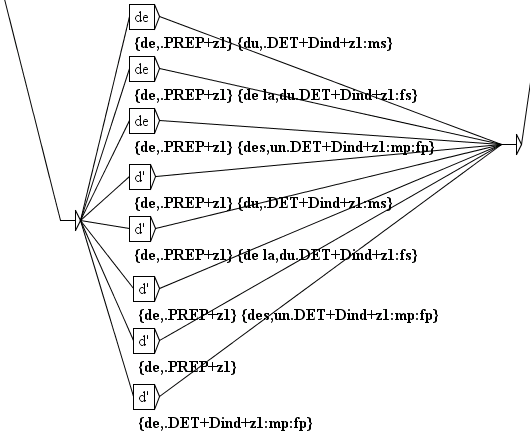
\includegraphics[width=13.5cm]{resources/img/fig6-3.png}
\caption{Extrait du graphe de normalisation utilisé pour le
français\label{fig-tfst-normalization-grammar}}
\end{center}
\end{figure}

\noindent Les chemins décrivent les formes qui doivent être normalisées. Les variantes minuscules
et majuscules sont prises en compte selon le principe suivant : les lettres majuscules dans
le graphe ne reconnaissent que les lettres majuscules dans l’automate du texte ; les lettres
minuscules peuvent reconnaître les lettres minuscules et majuscules.\index{Respect de la casse}

\bigskip
\noindent Les sorties représentent les séquences d’étiquettes qui seront insérées dans l’automate
du texte. Ces étiquettes peuvent être des entrées de dictionnaires ou de simples chaînes
de caractères. Les étiquettes représentant des entrées de dictionnaire doivent respecter le
format des entrées d’un DELAF et être encadrées par les symboles
\verb+{+ et \verb+}+. Les sorties à variables n’ont pas de sens dans ce type de graphe.


\bigskip
\noindent Il est possible de faire appel à des sous-graphes. Il n’est pas possible de faire référence
aux dictionnaires pour décrire les formes à normaliser. L’unique symbole spécial reconnu
dans ce type de graphe est le mot vide \verb+<E>+.\index{\verbc{<E>}}
Les graphes de normalisation de formes ambiguës doivent être compilés avant de pouvoir être
utilisés.


\subsection{Graphes syntaxiques}
\label{syntactic-graphs}\index{Graphe!syntaxique}\index{Grammaires!locales}
Les graphes syntaxiques, également appelés grammaires locales, permettent de décrire
des motifs syntaxiques qui pourront ensuite être recherchés dans des textes. De tous les
types de graphe, ceux-ci possèdent la plus grande puissance d’expressions, car ils permettent
de faire référence aux dictionnaires.\index{Référence aux informations dans les dictionnaires}
\index{Dictionnaire!référence aux informations du}

\bigskip
\noindent Les variantes minuscules/majuscules sont autorisées selon le principe décrit plus haut.
Il est toutefois possible de forcer le respect de la casse en encadrant une expression avec des
guillemets. L’emploi des guillemets permet également de forcer le respect des espacements.
En effet, Unitex considère, par défaut, qu’un espace est possible entre deux boîtes. Pour forcer
la présence d’un espace, il faut le mettre entre guillemets. Pour interdire la présence d’un
espace, il faut utiliser le symbole spécial \verb+#+.\index{\verbt{\#}}
\index{Respect!des minuscules/majuscules}\index{Casse!voir {Respect!des minuscules/majuscules}}
\index{Minuscules!voir {Respect!de minuscules/majuscules}}
\index{Majuscules!voir {Respect!de minuscules/majuscules}}
\index{Respect!des espaces}

\bigskip
\noindent Les graphes syntaxiques peuvent faire appel à des sous-graphes (voir section
~\ref{section-subgraphs}). Ils gèrent également les sorties, y compris les sorties à variables.
Les séquences produites sont interprétées comme des chaînes de caractères qui seront insérées
dans les concordances ou dans le texte si vous voulez modifier celui-ci (voir section
~\ref{section-modifying-text}).

\bigskip
\noindent Les graphes syntaxiques peuvent utiliser des contextes (voir section~\ref{section-contexts}).

\bigskip
\noindent Les graphes syntaxiques peuvent utiliser des filtres morphologiques (voir section
\ref{section-filters}).

\bigskip
\noindent Les graphes syntaxiques peuvent utiliser le mode morphologique (voir section
\ref{section-morphological-mode}).

\bigskip
\noindent Les symboles spéciaux supportés par les graphes syntaxiques sont les mêmes que ceux
utilisables dans les expressions rationnelles (voir section~\ref{section-special-symbols}).

\bigskip
\noindent Il n’est pas obligatoire de compiler les graphes syntaxiques avant de les utiliser pour la
recherche de motifs. Si un graphe n’est pas compilé, le système le compilera automatiquement.


\subsection{Grammaires ELAG}
\index{Grammaires!ELAG}\index{ELAG}

La syntaxe des grammaires de levée d’ambiguïtés est présentée à la section \ref{section-elag-grammars},
page \pageref{section-elag-grammars}.


\subsection{Graphes paramétrés}
\index{Graphe!paramétré}
Les graphes paramétrés sont des méta-graphes permettant de générer une famille de
graphes à partir d’une table de lexique-grammaire. Il est possible de construire des graphes
paramétrés pour n’importe quel type de graphe. La construction et l’utilisation des graphes
paramétrés seront développées dans le chapitre
~\ref{chap-lexicon-grammar}.

\section{Compilation d'une grammaire}
\label{section-graph-compilation}
\subsection{Compilation d'un graphe}
\index{Graphe!compilation}\index{Compilation!d'un graphe}
La compilation est l’opération qui permet de passer du format \verb+.grf+ à un format plus
facile à manipuler par les programmes d’Unitex. Pour compiler un graphe, vous devez
l’ouvrir, puis cliquer sur "Compile FST2" dans le sous-menu "Tools" du menu "FSGraph".
Unitex lance alors le programme \verb+Grf2Fst2+\index{\verbc{Grf2Fst2}}\index{Programmes externes!\verbc{Grf2Fst2}} dont vous pouvez suivre l’exécution dans une fenêtre
(voir figure~\ref{fig-compilation-frame}).

\bigskip
\begin{figure}[!ht]
\begin{center}
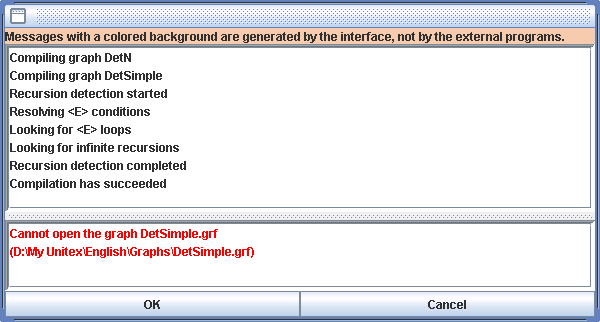
\includegraphics[width=14.7cm]{resources/img/fig6-4.png}
\caption{Fenêtre de compilation\label{fig-compilation-frame}}
\end{center}
\end{figure}

\noindent Si le graphe fait appel à des sous-graphes, ceux-ci sont automatiquement compilés. Le
résultat est un fichier \verb+.fst2+ fichier\index{Fichier!\verbc{.fst2}} qui rassemble tous les
graphes qui composent la grammaire. La grammaire est alors prête à être utilisée par les
différents programmes d’Unitex.


\subsection{Approximation par un transducteur fini}
\index{Graphe!approximation par transducteur fini}
\index{Approximation d'une grammaire par un transducteur fini}
\index{\verbc{Flatten}}\index{Programmes externes!\verbc{Flatten}}\label{flatten-section}
Le format FST2 conserve l’architecture en sous-graphes des grammaires, ce qui les différencie
des stricts transducteurs à états finis. Le programme \verb+Flatten+ permet de transformer
une grammaire FST2 en un transducteur à états finis quand cela est possible, et d’en
construire une approximation dans le cas contraire. Cette fonction permet ainsi d’obtenir des objets
plus simples à manipuler et sur lesquels peuvent s’appliquer tous les algorithmes classiques sur
les automates.


\bigskip
\noindent Pour compiler et transformer ainsi une grammaire, sélectionnez la commande "Compile
Flatten FST2" dans le sous-menu "Tools" du menu "FSGraph". La fenêtre de la figure~\ref{fig-flatten-configuration}
vous permet de configurer l’opération d’approximation.

\bigskip
\begin{figure}[!ht]
\begin{center}
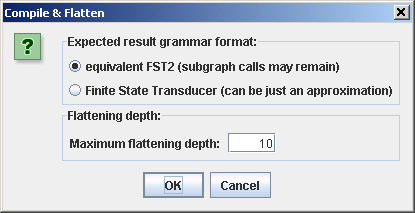
\includegraphics[width=10.4cm]{resources/img/fig6-5.png}
\caption{Configuration de l’approximation d’une grammaire\label{fig-flatten-configuration}}
\end{center}
\end{figure}

\noindent Le cadre "Flattening depth" permet de préciser le niveau d’imbrication des sous-graphes.
Cette valeur représente la profondeur maximale au-delà de laquelle les appels à des sous-
graphes ne seront plus remplacés par les sous-graphes eux-mêmes.


\bigskip
\noindent Le cadre "Expected result grammar format" permet de déterminer le comportement du
programme au-delà de la limite indiquée. Si vous sélectionnez l’option "Finite State Transducer",
les appels aux sous-graphes seront ignorés (remplacé par \verb+<E>+) au-delà de la profondeur
maximale. Cette option garantit ainsi l’obtention d’un transducteur à états finis, éventuellement
non équivalent à la grammaire de départ. En revanche, l’option "equivalent FST2" indique au
programme de laisser tels quels les appels aux sous-graphes au-delà de la profondeur limite.
Cette option garantit la stricte équivalence du résultat avec la grammaire d’origine, mais
ne produit pas forcément un transducteur à états finis. Cette option peut être utilisée pour
optimiser certaines grammaires.


\bigskip
\noindent Un message indique à la fin du processus d’approximation si le résultat est un transducteur
à états finis ou une grammaire FST2, et dans le cas d’un transducteur, s’il est équivalent
à la grammaire d’origine (voir figure~\ref{fig-flatten-result}).


\bigskip
\begin{figure}[!ht]
\begin{center}
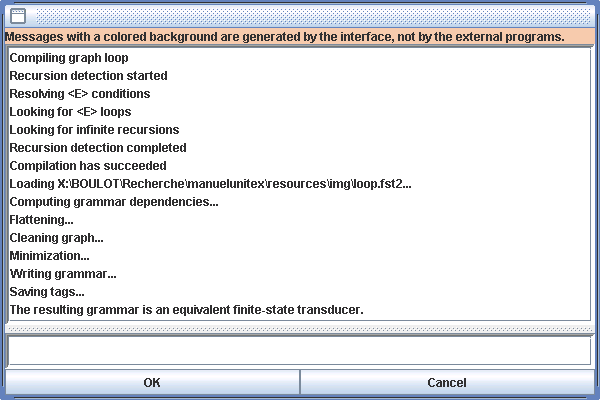
\includegraphics[width=14.7cm]{resources/img/fig6-6.png}
\caption{Résultat de l’approximation d’une grammaire\label{fig-flatten-result}}
\end{center}
\end{figure}


\subsection{Contraintes sur les grammaires}
\index{Grammaires!contraintes}\index{Contraintes sur les grammaires}
À l’exception des grammaires de flexion, une grammaire ne peut pas avoir de chemin
vide. Cela signifie que le graphe principal d’une grammaire ne doit pas pouvoir reconnaître
le mot vide, mais cela n’empêche pas un sous-graphe de cette grammaire de reconnaître
epsilon.


\bigskip
\noindent Il n’est pas possible d’associer une sortie à un appel à un sous-graphe. De telles sorties
sont ignorées par Unitex. Il faut donc utiliser une boîte vide située immédiatement à gauche
de l’appel au sous-graphe pour porter la sortie (voir figure~\ref{fig-subgraph-output}).
\index{Sortie d'un transducteur!associée à un appel de sous-graphe}

\bigskip
\begin{figure}[!ht]
\begin{center}
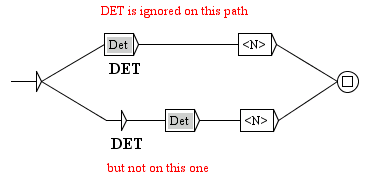
\includegraphics[width=9.1cm]{resources/img/fig6-7.png}
\caption{Comment associer une sortie à un appel de sous-graphe\label{fig-subgraph-output}}
\end{center}
\end{figure}

\index{Boucles sans fin}
\noindent Les grammaires ne doivent pas non plus comporter de boucles infinies, car les programmes
d’Unitex ne pourraient jamais terminer l’exploration de telles grammaires.
%A void loop is a configuration that causes the \verb+Locate+ program to enter an infinite loop.
Ces boucles peuvent être dues à des transitions étiquetées par le mot vide epsilon ou à des
appels de sous-graphes récursifs.


\bigskip
\noindent Les boucles dues à des transitions par le mot vide peuvent avoir deux origines dont la
première est illustrée par la figure~\ref{fig-epsilon-output-loop}.
Ce type de boucle est dû au fait qu’une transition par le mot vide ne peut pas être éliminée
automatiquement par Unitex lorsqu’elle est munie d’une sortie. Ainsi, la transition par
le mot vide de la figure~\ref{fig-epsilon-output-loop} ne sera pas supprimée et provoquera une
boucle infinie.

\bigskip
\begin{figure}[!ht]
\begin{center}
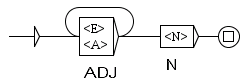
\includegraphics[width=6.2cm]{resources/img/fig6-8.png}
\caption{Boucle infinie due à une transition par le mot vide avec sortie\label{fig-epsilon-output-loop}}
\end{center}
\end{figure}

\bigskip
\noindent La seconde catégorie de boucle par epsilon concerne les appels à des sous-graphes pouvant
reconnaître le mot vide. Ce cas de figure est illustré par la
figure~\ref{fig-epsilon-subgraph-loop}: si le sous-graphe \verb+Adj+ reconnait epsilon, on a une
boucle infinie qu’Unitex ne peut pas éliminer.

\bigskip
\begin{figure}[!ht]
\begin{center}
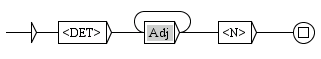
\includegraphics[width=7.9cm]{resources/img/fig6-9.png}
\caption{Boucle infinie due à un appel à un sous-graphe reconnaissant epsilon
\label{fig-epsilon-subgraph-loop}}
\end{center}
\end{figure}

\begin{figure}[!ht]
\begin{center}
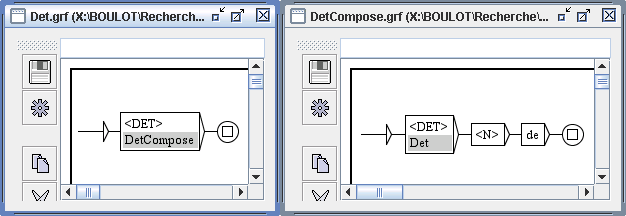
\includegraphics[width=15.5cm]{resources/img/fig6-10.png}
\caption{Boucle infinie causée par deux graphes s'appelant l'un l'autre
\label{fig-recursive-calls-loop}}
\end{center}
\end{figure}

\noindent La troisième possibilité de boucle infinie concerne les appels récursifs à des
sous-graphes. Considérons les graphes \verb+Det+ et \verb+DetCompose+ de la
figure~\ref{fig-recursive-calls-loop}.
 Chacun de ces graphes peut appeler l’autre \textit{sans rien lire dans le texte}. Le fait qu’aucun
 des deux graphes ne comporte d’étiquette entre l’état initial et l’appel à l’autre graphe est
 capital. En effet, s’il y avait au moins une étiquette différente d’epsilon entre le début du
 graphe \verb+Det+ et l’appel à \verb+DetCompose+, cela signifierait que les programmes d’Unitex
 explorant le graphe \verb+Det+ devraient lire le motif décrit par cette étiquette dans le texte
 avant d’appeler récursivement \verb+DetCompose+ Dans ce cas, les programmes ne pourraient boucler
 indéfiniment que s’ils rencontraient une infinité de fois le motif dans le texte, ce qui ne peut
 pas arriver.

\pagebreak
\subsection{Intervalle pour le nombre de répétitions}
\label{nb-repetitions}\index{Intervalle}\index{Boucle!nombre de répétitions}\index{Nombre de répétitions}\index{Répétition!nombre de}
\noindent Pour reconnaître des séquences de tokens dans laquelle un motif apparaît une fois, plusieurs fois
ou jamais, on peut associer un intervalle d'entiers à une boîte. Cela fixe les limites du nombre de fois
que le motif apparait. Le motif doit être décrit dans une boite unique.
Si on associe un intervalle  [m,M]  à une boîte contenant <A> (figure~\ref{intervals}), le chemin reconnaitra des séquences avec au moins $m$ adjectifs consécutifs et pas plus de $M$.

\begin{figure}[h!]
\begin{center}
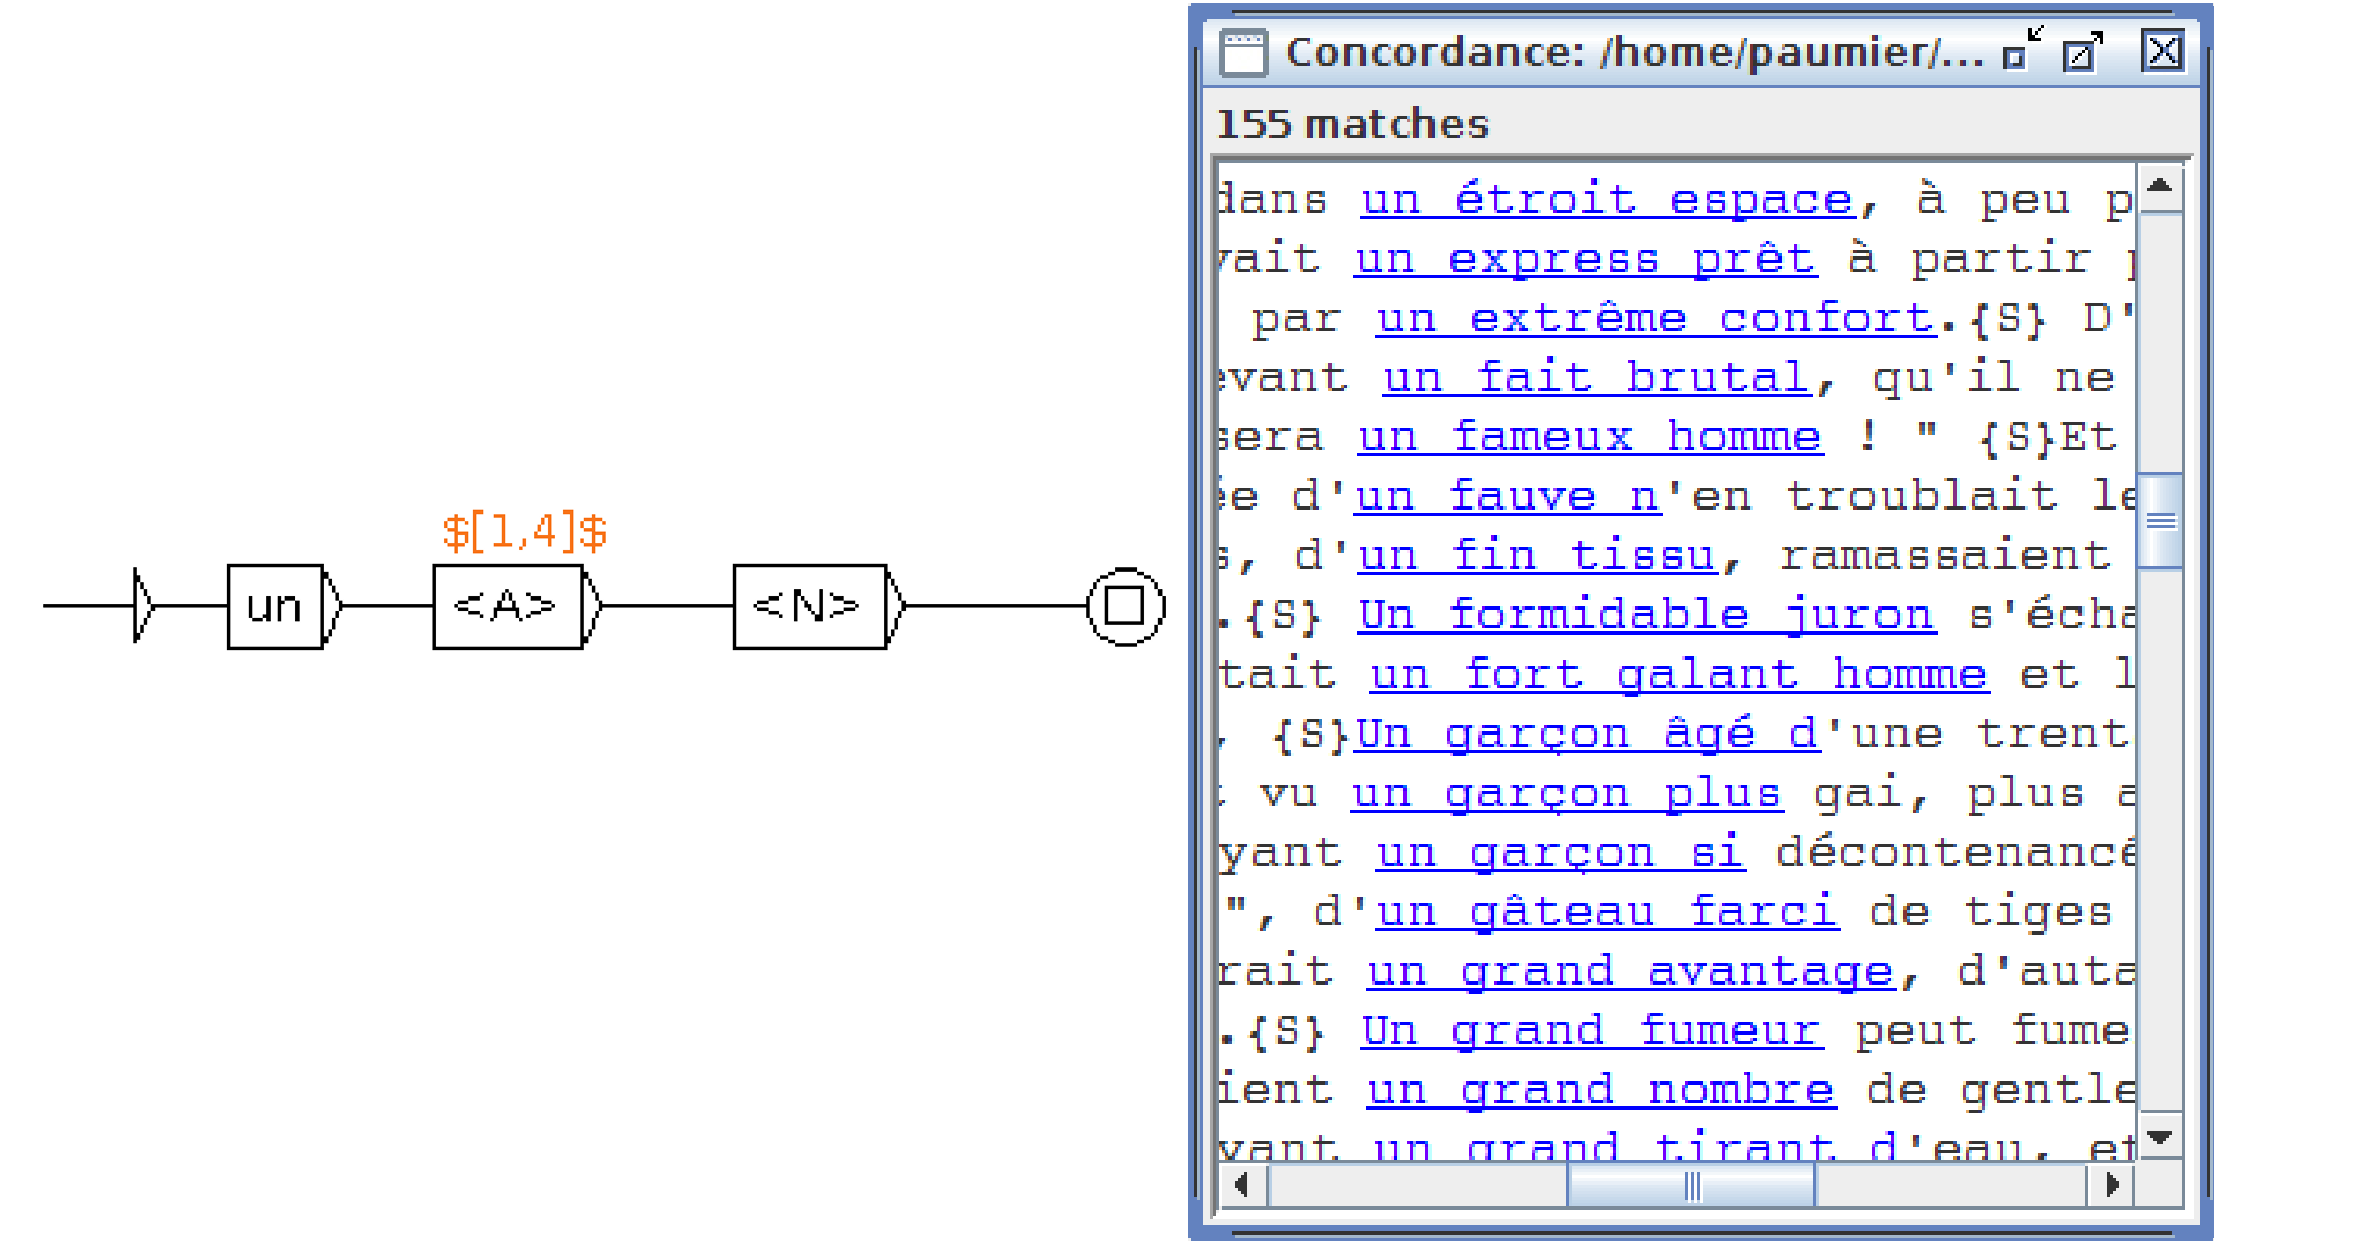
\includegraphics[width=13.5cm]{resources/img/fig6-10a.png}
\caption{Utilisation d'un intervalle pour reconnaître plusieurs tokens consécutifs\label{intervals}}
\end{center}
\end{figure}

\noindent  On attache un intervalle en insérant \verb+$[m,M]$+ dans la sortie de la boite,
juste après le caractère ``/'', et selon les règles : 
\begin{itemize}
\item \verb+[m,M]+ = au moins $m$ motifs consécutifs et pas de plus de $M$
\item \verb+[,M]+ = de 0 à $M$  
\item \verb+[m,]+ = au moins $m$
\end{itemize}

\noindent La boite ne doit pas être connectée à elle-même par une boucle directe. Un intervalle est compatible avec 
une sortie au sens habituel. Par exemple, pour insérer sous la boite de la figure~\ref{intervals}
la sortie \verb+<ADJ position='antéposé'>+, saisissez  dans le champ
texte~: \verb+<A>/$[1,4]$/<ADJ position='antéposé'>+. 

\subsection{Détection d’erreurs}
\index{Détection d'erreur dans les graphes}\index{Graphe!détection d'erreur}
\index{Erreurs dans les graphes}
Pour éviter aux programmes de se bloquer ou de planter, Unitex effectue automatique-
ment une détection d’erreurs lors de la compilation des graphes. Le compilateur de graphes
vérifie que le graphe principal ne reconnaît pas le mot vide et recherche toutes les formes de
boucles infinies. Si une erreur est trouvée, un message d’erreur apparaît dans la fenêtre de
compilation. La figure ~\ref{fig-error-message} montre le message obtenu lorsqu’on tente de 
compiler le graphe \verb+Det+ de la figure~\ref{fig-recursive-calls-loop}.

\begin{figure}[!ht]
\begin{center}
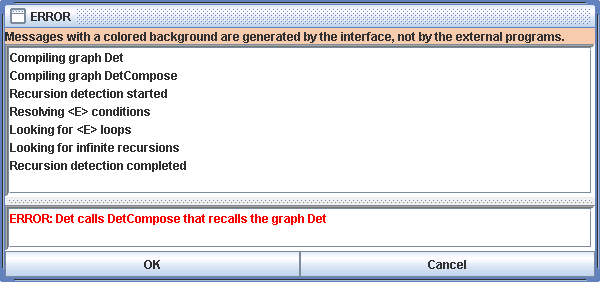
\includegraphics[width=15cm]{resources/img/fig6-11.png}
\caption{Message d’erreur obtenu en compilant le graphe
\texttt{Det}\label{fig-error-message}}
\end{center}
\end{figure}

\noindent Si vous avez lancé une recherche de motifs en sélectionnant un graphe au format 
\verb+.grf+ \index{Fichier!\verbc{.grf}}, et qu’Unitex y décèle une erreur, l’opération
de recherche sera automatiquement interrompue.


\section{Contextes}
\index{Contexte!zone dans un graphe}\label{section-contexts}

Les graphes d’Unitex sont des grammaires algébriques. Elles sont également appelées
grammaires hors-contexte, car lorsque l’on souhaite reconnaître une séquence
 $A$, on ne tient pas compte du contexte dans lequel $A$ apparaît. Par exemple, il est 
 impossible de rechercher avec un graphe normal toutes les occurrences du mot \verb+president+, 
 sauf celles qui sont suivies par \verb+of the republic+.


\bigskip
\noindent Il est toutefois possible de tenir compte du contexte dans les graphes syntaxiques. Dans
ce cas, les graphes ne sont plus des grammaires algébriques, mais des grammaires contex-
tuelles qui n’ont pas les mêmes propriétés théoriques.
.

\subsection{Contextes droits}
\index{\verbc{$[}}
\index{\verbc{$]}}
On définit un contexte droit en délimitant une zone du graphe avec des boîtes contenant
\verb+$[+ and \verb+$]+, représentant respectivement les début et fin de contexte qui sont
représentés dans le graphe par des crochets verts. Le début et la fin d’un contexte doivent
apparaître dans le même graphe.


\bigskip
\begin{figure}[!ht]
\begin{center}
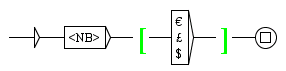
\includegraphics[width=7.4cm]{resources/img/fig6-12.png}
\caption{Utilisation d’un contexte droit\label{fig-context1}}
\end{center}
\end{figure}

\bigskip
\noindent La figure~\ref{fig-context1} montre un exemple simple de contexte. Ce graphe
reconnaît tous les nombres qui sont suivis par l’euro, la livre ou le dollar, mais sans
que le symbole d’unité n’apparaisse dans les occurrences trouvées, c'est-à-dire dans
la concordance.

\bigskip
\noindent Les contextes s’interprètent de la façon suivante. Supposons que l’on rencontre un début
de contexte lors de l’application d’une grammaire à un texte, et notons $pos$ la position courante
dans le texte à cet instant. Le programme \verb$Locate$ va ensuite chercher à reconnaître
l’expression décrite dans le contexte. S’il échoue, il n’y aura pas de match. S’il réussit, c’est-
à-dire s’il peut atteindre la fin du contexte, le programme reviendra à la position $pos$ dans
le texte et continuera l’exploration de la grammaire à partir de la fin du contexte.

\bigskip
\noindent Les poids (section~\ref{Transducers}) dans les contextes droits sont ignorés.

\bigskip
\noindent On peut également définir des contextes droits négatifs, en utilisant
 \verb+$![+ comme début de contexte. La figure~\ref{fig-context2}
montre un graphe reconnaissant des nombres qui ne sont pas suivis par \verb+th+.
 La différence avec les contextes positifs est que lorsque \verb$Locate$ essaie de reconnaître
 l’expression décrite dans le contexte, le fait d’atteindre la fin du
 contexte est considéré comme un échec, car cela signifie que l’on a reconnu une séquence interdite.
 À l’inverse, si la fin de contexte ne peut être atteinte, le programme \verb$Locate$ reviendra à
 la position $pos$ dans le texte et continuera l’exploration de la grammaire à partir de la fin du
 contexte.

\begin{figure}[!ht]
\begin{center}
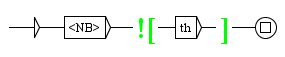
\includegraphics[width=7.3cm]{resources/img/fig6-13.png}
\caption{Utilisation d’un contexte négatif\label{fig-context2}}
\end{center}
\end{figure}

\bigskip
\noindent Les contextes peuvent être placés n’importe où dans le graphe, y compris au début. La
figure~\ref{fig-context3} montre ainsi un graphe qui reconnaît un adjectif dans le contexte de
quelque
chose qui n’est pas un participe passé. Autrement dit, ce graphe reconnaît tous les adjectifs
qui ne sont pas ambigus avec des participes passés.

\begin{figure}[!ht]
\begin{center}
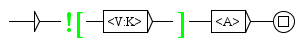
\includegraphics[width=7.5cm]{resources/img/fig6-14.png}
\caption{Recherche d’un adjectif non ambigu avec un participe passé\label{fig-context3}}
\end{center}
\end{figure}

\bigskip
\noindent Dans les graphes tels que celui de la figure~\ref{fig-context3}, le contexte droit négatif
ne vérifie pas nécessairement le même nombre de tokens que la boite qui le suit. Par exemple, avant
que le graphe de la figure~\ref{too-also} ne reconnaisse \verb+too+, le contexte droit négatif
vérifie s'il apparait dans une expression telle que \verb+too early+ ou \verb+too many+.

\begin{figure}[!ht]
\begin{center}
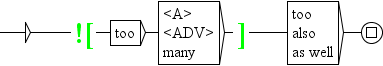
\includegraphics[width=7.5cm]{resources/img/fig-too-also.png}
\caption{Un contexte qui ne vérifie pas le même nombre de mots que la boite qui le suit\label{too-also}}
\end{center}
\end{figure}

\bigskip
\noindent On peut formuler des requêtes complexes avec les contextes droits négatifs. Ainsi, la figure
~\ref{fig-context4} montre un graphe qui reconnaît toutes les séquences de deux noms simples qui ne
sont pas ambiguës avec des mots composés. En effet, le motif \verb?<CDIC><<^([^ ]+ [^ ]+)$>>? 
reconnaît un mot composé contenant exactement un espace, et le motif \verb?<N><<^([^ ]+)$>>?
reconnaît un nom sans espace, c’est-à-dire un nom simple. Ainsi,
 dans la phrase \textit{Black cats should like the town hall}, ce graphe reconnaîtra
 \textit{Black cats}, mais pas \textit{town hall}, qui est un mot composé.

\bigskip
\begin{figure}[!ht]
\begin{center}
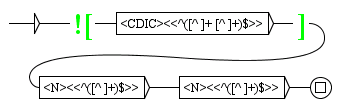
\includegraphics[width=8.9cm]{resources/img/fig6-15.png}
\caption{Utilisation avancée des contextes\label{fig-context4}}
\end{center}
\end{figure}

\bigskip
\noindent Il est possible d’imbriquer des contextes. Par exemple, le graphe de la
figure~\ref{fig-context5}
reconnaît un nombre qui n’est pas suivi par un point, sauf si ce point est suivi par un nombre.
Ainsi, dans le texte \textit{5.0+7.=12}, ce graphe reconnaîtra \textit{5}, \textit{0} et
\textit{12}.

\bigskip
\begin{figure}[!ht]
\begin{center}
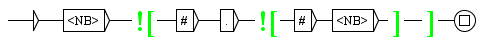
\includegraphics[width=12cm]{resources/img/fig6-16.png}
\caption{Imbrication de contextes\label{fig-context5}}
\end{center}
\end{figure}

\bigskip
\noindent Les sorties qui se trouvent dans des boîtes à l’intérieur d’un contexte sont ignorées.
En revanche, il est possible d’utiliser une variable qui a été définie dans un contexte, comme
c’est le cas sur la figure ~\ref{fig-context6}). Si l’on applique ce graphe en mode MERGE au texte
\textit{the cat is white}, on obtient en sortie :

\bigskip
\texttt{the \textcolor{blue}{<pet name="cat" color="white"/>} is white}

\bigskip

\begin{figure}[!ht]
\begin{center}
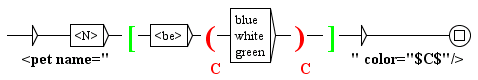
\includegraphics[width=12.2cm]{resources/img/fig6-17.png}
\caption{Variable définie dans un contexte\label{fig-context6}}
\end{center}
\end{figure}

\subsection{Contextes gauches}
\index{\verbc{$*}}
Il est également possible de rechercher une expression $X$ si elle se trouve seulement après une 
expression $Y$. Évidemment, il était déjà possible de le faire avec une grammaire semblable à celle
de la figure \ref{fig-left-context1}. Cependant, avec ce type de grammaire, le contexte gauche est
inclus dans la séquence reconnue, comme le montre la figure~\ref{fig-left-context2}.

\begin{figure}[!ht]
\begin{center}
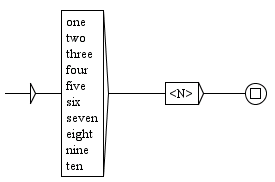
\includegraphics[width=7cm]{resources/img/fig6-17a.png}
\caption{Reconnaissance d'un nom précédé d'un déterminant numéral\label{fig-left-context1}}
\end{center}
\end{figure}

\begin{figure}[!ht]
\begin{center}
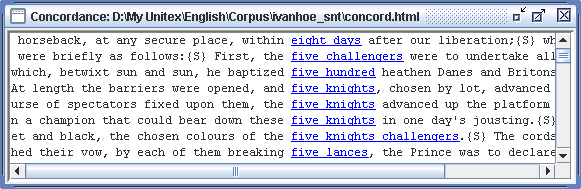
\includegraphics[width=14cm]{resources/img/fig6-17b.png}
\caption{Résultats de l'application de la grammaire de la figure
\ref{fig-left-context1}\label{fig-left-context2}}
\end{center}
\end{figure}

\bigskip
\noindent Pour éviter cela, on peut utiliser le symbole \verb+$*+ qui indique la fin du contexte
gauche de l'expression qu'on désire reconnaître. Ce symbole est représenté par une étoile verte
dans le graphe, comme le montre la figure~\ref{fig-left-context3}. L'effet d'un tel contexte est
d'utiliser une partie de la grammaire pour calculer la séquence reconnue, sans que cette partie ne figure dans le résultat (voir figure~\ref{fig-left-context4}).

\begin{figure}[!ht]
\begin{center}
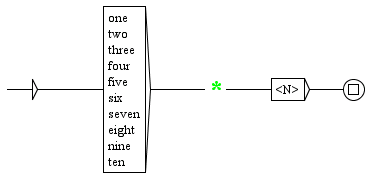
\includegraphics[width=9cm]{resources/img/fig6-17c.png}
\caption{Reconnaissance d'un nom après un contexte gauche\label{fig-left-context3}}
\end{center}
\end{figure}

\begin{figure}[!ht]
\begin{center}
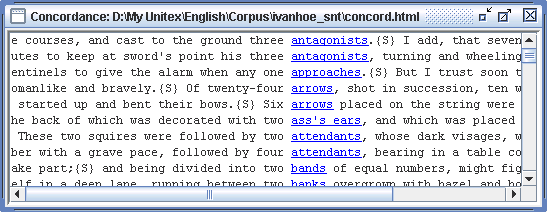
\includegraphics[width=14cm]{resources/img/fig6-17d.png}
\caption{Résultats de l'application de la grammaire de la figure
\ref{fig-left-context3}\label{fig-left-context4}}
\end{center}
\end{figure}

\clearpage
\noindent Toutes les sorties produites par un contexte gauche sont ignorées, comme on peut le voir dans la concordance de la figure \ref{fig-left-context6}, qui donne les résultats
obtenus avec la grammaire de la figure \ref{fig-left-context5}.

\begin{figure}[!ht]
\begin{center}
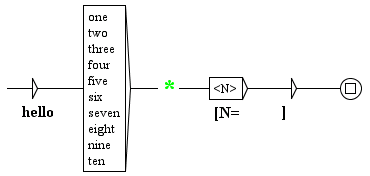
\includegraphics[width=9cm]{resources/img/fig6-17e.png}
\caption{Sorties ignorées dans un contexte gauche\label{fig-left-context5}}
\end{center}
\end{figure}

\begin{figure}[!ht]
\begin{center}
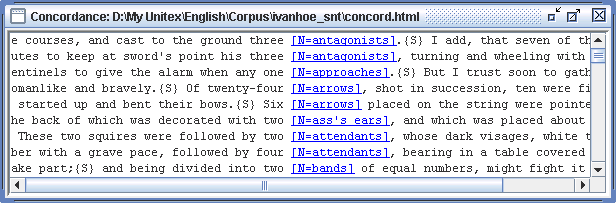
\includegraphics[width=15cm]{resources/img/fig6-17f.png}
\caption{Résultats de l'application de la grammaire de la figure
\ref{fig-left-context5}\label{fig-left-context6}}
\end{center}
\end{figure}

\bigskip
\noindent Toutefois, on peut mémoriser des informations avec des variables (voir section
\ref{section-variables}) et les utiliser en dehors du contexte gauche, comme le montrent la
grammaire de la figure~\ref{fig-left-context7} et son résultat dans la figure~\ref{fig-left-context8}.

\begin{figure}[!ht]
\begin{center}
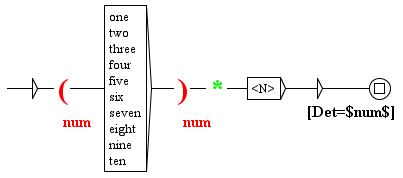
\includegraphics[width=10cm]{resources/img/fig6-17g.png}
\caption{Utilisation d'une variable dans un contexte gauche\label{fig-left-context7}}
\end{center}
\end{figure}

\begin{figure}[!ht]
\begin{center}
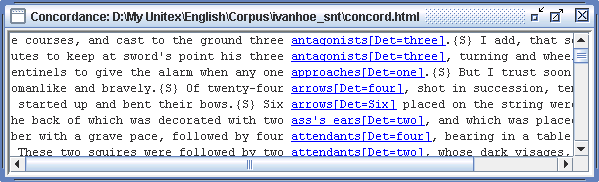
\includegraphics[width=15cm]{resources/img/fig6-17h.png}
\caption{Résultats de l'application de la grammaire de la figure
\ref{fig-left-context7}\label{fig-left-context8}}
\end{center}
\end{figure}

\bigskip
\noindent On peut invoquer dans une grammaire un graphe qui contient des contextes gauches,
mais cela nécessite d'être vigilant. Au moment où le contexte gauche est exclu de la séquence reconnue,
toutes les séquences qui avaient été reconnues par des graphes appelants en sont exclues également,
car la séquence qui sera finalement reconnue devra être contiguë. Les sorties correspondant aux
séquences exclues sont ignorées elles aussi.

\bigskip
\noindent Ainsi, avec des contextes gauche et droit, on peut faire une distinction entre les motifs
utilisés pour reconnaître des points du texte, et la délimitation des séquences à extraire dans les 
résultats. Par exemple, la grammaire de la figure \ref{fig-left-context9} cherche des
expressions comme \verb$the animal's$, mais extrait seulement les noms, comme on peut le voir
figure \ref{fig-left-context10}.

\begin{figure}[!ht]
\begin{center}
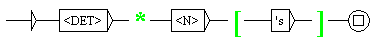
\includegraphics[width=10cm]{resources/img/fig6-17i.png}
\caption{Une grammaire avec des contextes gauche et droit\label{fig-left-context9}}
\end{center}
\end{figure}

\begin{figure}[!ht]
\begin{center}
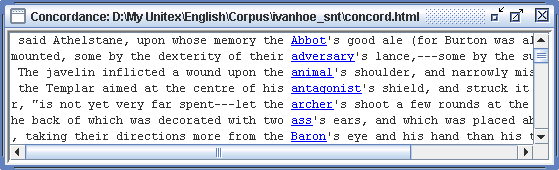
\includegraphics[width=15cm]{resources/img/fig6-17j.png}
\caption{Résultats de l'application de la grammaire de la figure
\ref{fig-left-context9}\label{fig-left-context10}}
\end{center}
\end{figure}

\bigskip
\noindent Les poids (section~\ref{Transducers}) fonctionnent normalement dans les contextes gauches.

\clearpage

\section{Le mode morphologique}
\label{section-morphological-mode}
\index{Mode morphologique}
\subsection{Pourquoi ?}
Comme Unitex fonctionne sur une version "tokenisée" du texte, il n'est pas possible de
faire des requêtes qui entrent à l'intérieur des "tokens", sauf avec les filtres morphologiques
(voir section \ref{section-filters}), comme le montre la figure
\ref{fig-morpho1}.

\begin{figure}[!ht]
\begin{center}
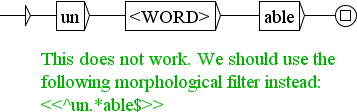
\includegraphics[width=7cm]{resources/img/fig6-17k.png}
\caption{Reconnaissance d'éléments morphologiques\label{fig-morpho1}}
\end{center}
\end{figure}

\bigskip
\noindent Cependant, les filtres morphologiques ne permettent pas n'importe quelle requête, puisqu'ils ne
peuvent pas faire référence aux informations contenues dans les dictionnaires. Ainsi, il est impossible de formuler de cette 
manière une requête comme ``\textit{un mot constitué du préfixe} \verb$un$ \textit{suivi d'un adjectif en} \verb+able+''.

\bigskip
\noindent Pour surmonter cette difficulté, nous introduisons un mode morphologique dans le programme
\verb$Locate$. Il consiste à délimiter une partie de votre  grammaire avec les 
symboles \verb+$<+ et \verb+$>+.\index{\verbc{$<}}\index{\verbc{$>}}
Dans cette zone, les données sont reconnues lettre par lettre, comme le montre la figure
\ref{fig-morpho2}.

\begin{figure}[!ht]
\begin{center}
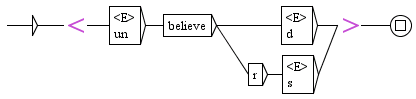
\includegraphics[width=11cm]{resources/img/fig6-17l.png}
\caption{Exemple de zone morphologique dans la grammaire\label{fig-morpho2}}
\end{center}
\end{figure}

\subsection{Les règles}
Dans ce mode, le contenu du graphe n'est pas interprété de manière habituelle.
\begin{enumerate}
\item Il n'y a pas d'espace entre les boîtes. Ainsi, si on désire reconnaître un espace,
	on doit le rendre explicite avec \verb+" "+ (un espace entre guillemets).

\item On peut toujours utiliser des sous-graphes, mais la fin de la zone morphologique
	doit se trouver dans le même graphe que son début.

\item On peut utiliser des masques lexicaux qui nécessitent la consultation d'un dictionnaire
--- comme \verb+<DIC>+ , \verb+<be>+ ou \verb+<N:ms>+, qui font référence aux informations contenues dans un dictionnaire ---, du moment qu'il a été préalablement déclaré comme dictionnaire
du mode morphologique (voir section~\ref{dic-mode-morpho}). 
   
\item On peut utiliser des masques lexicaux qui nécessitent la consultation d'un graphe-dictionnaire
(section~\ref{section-dictionary-graphs}), du moment que le nom du graphe-dictionnaire contient l'option \verb+b+.
Cependant, cette possibilité ne fonctionne que pour les formes reconnues dans le texte par le graphe-dictionnaire
pendant l'application initiale des dictionnaires (section~\ref{section-applying-dictionaries}),
et non pour les formes qui n'apparaissent dans le texte que comme des parties de tokens.
   
\item On peut utiliser des filtres morphologiques (section~\ref{section-filters}). Cependant, les filtres
           morphologiques employés seuls ou sur \verb+<TOKEN>+
	ne s'appliqueront seulement qu'au caractère courant. Par 
	conséquent, les filtres comme \verb+<<[1-9][0-9]>>+ qui sont conçus pour reconnaître plus d'un
	caractère ne reconnaîtront jamais rien. En fait, dans le mode morphologique, 
	les filtres morphologiques ne sont utiles que pour exprimer des négations
	comme \verb+<<[^aeiouy]>>+ (n'importe quel caractère qui n'est pas une voyelle). 
   
\item Les contextes gauches et droits au sens de la section~\ref{section-contexts} sont interdits.

\item On peut utiliser des sorties.
   
\item \verb+<LETTRE>+ reconnaît n'importe quelle lettre définie dans le fichier alphabet.
	\index{\verbc{<MOT>}}\index{\verbc{<LETTER>}}

\item \verb+<MIN>+ reconnaît n'importe quelle minuscule définie dans le fichier alphabet.\index{\verbc{<MIN>}}\index{\verbc{<LOWER>}}

\item \verb+<MAJ>+ reconnaît n'importe quelle majuscule définie dans le fichier alphabet.\index{\verbc{<MAJ>}}\index{\verbc{<UPPER>}}

\item \verb+<DIC>+ reconnaît n'importe quel mot présent dans un dictionnaire du mode
	 morphologique\index{\verbc{<DIC>}}, mais les méta-symboles \verb+#+, \verb+<PRE>+,  \verb+<NB>+,
 	 \verb+<SDIC>+ et\verb+<CDIC>+ sont interdits.\index{\verbt{\#}} \index{\verbc{<FIRST>}} \index{\verbc{<NB>}} \index{\verbc{<TOKEN>}} \index{\verbc{<SDIC>}} \index{\verbc{<CDIC>}}
\item Si on atteint la fin de la zone sans être à la fin du token, la reconnaissance échoue.
	Par exemple, si le texte contient \verb+enabled+, on ne peut pas reconnaître seulement
	\verb+enable+.
\end{enumerate}

\noindent  Il est également possible d'utiliser de manière alternative  les codes anglais \verb+<WORD>+, \verb+<LOWER>+, \verb+<UPPER>+ et \verb+<FIRST>+
respectivement à la place de \verb+<MOT>+, \verb+<MIN>+, \verb+<MAJ>+ et \verb+<PRE>+ si vous réalisez des grammaires dans cette langue.

\subsection{Dictionnaires du mode morphologique}
\index{Dictionnaire!du mode morphologique}
\label{dic-mode-morpho}
Dans le mode morphologique, on peut faire des requêtes qui utilisent les dictionnaires.
Par exemple,  la grammaire de la figure \ref{fig-morpho3} cherche les mots constitués du préfixe \verb+un+ suivi d'un adjectif.

\begin{figure}[!ht]
\begin{center}
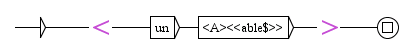
\includegraphics[width=11cm]{resources/img/fig6-17m.png}
\caption{Reconnaissance des mots constitués de \textit{un} et d'un adjectif en 
\textit{able}\label{fig-morpho3}}
\end{center}
\end{figure}

\begin{figure}[!ht]
\begin{center}
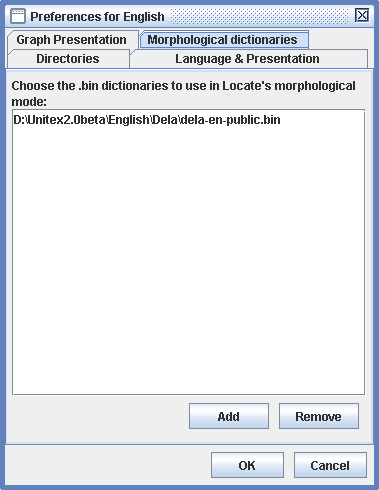
\includegraphics[width=11cm]{resources/img/fig6-17n.png}
\caption{Déclaration des dictionnaires du mode morphologique\label{fig-morpho4}}
\end{center}
\end{figure}

\bigskip
\noindent Pour pouvoir reconnaître le mot 
\verb+unaware+ avec cette grammaire, le système doit savoir que \verb+aware+ est un adjectif. 
Le masque lexical \verb+<A>+ nécessite la consultation d'un dictionnaire. Mais
\verb+aware+ peut ne pas être présent dans le texte, de sorte qu'on ne peut pas compter
sur les dictionnaires du texte\footnote{Les dictionnaires du texte sont compilés pendant l'application
initiale des dictionnaires (section~\ref{section-applying-dictionaries}), non pas pendant la recherche
de motifs.}.
C'est la raison pour laquelle on doit définir une liste de
dictionnaires à consulter en mode morphologique.
Pour ce faire, on va dans ``Info>Preferences>Morphological-mode dictionaries''
(figure~\ref{fig-morpho4}).
On peut définir autant de dictionnaires du mode morphologique qu'on veut, mais ils doivent
être au format \verb+.bin+. Ceci fait, on peut appliquer la grammaire.
Pour spécifier qu'un graphe-dictionnaire doit être consulté lorsqu'on est en mode morphologique,
on utilise l'option \verb+b+ ou \verb+z+ (section~\ref{section-dictionary-graphs}, Exporter les entrées produites
comme dictionnaire du mode morphologique).

\subsection{Variables de dictionnaire}
\index{Variable!de dictionnaire}
\index{Variable!morphologique}
\label{dictionary-variables}
On peut affecter à des variables des informations issues des dictionnaires du mode morphologique.
Ces variables sont appelées variables de dictionnaire ou variables morphologiques.
L'initialisation d'une variable de ce type doit être associée à une boite contenant un motif
qui fait référence à des informations contenues dans un dictionnaire du mode morphologique,
à l'exception du motif \verb+<DIC>+. On met \verb+$xxx$+ en sortie de la boîte, où \verb+xxx+ est un nom
correct de variable (cf. section~\ref{section-using-variables}). Ceci affecte à une  variable dénommée \verb+xxx+
l'entrée de dictionaire reconnue par le motif.
Dans la suite des chemins qui passent par la boite, on peut obtenir la forme fléchie, la forme canonique et les codes fournis par l'entrée avec
\verb+$xxx.INFLECTED$+, \verb+$xxx.LEMMA$+ et \verb+$xxx.CODE$+, comme le montre la figure
\ref{fig-morpho5}.
On peut également utiliser les motifs suivants:

\begin{itemize}
\item \verb+$xxx.CODE.GRAM$+: fournit seulement le premier code grammatical,
	censé être la catégorie grammaticale
  
\item \verb+$xxx.CODE.SEM$+: fournit tous les autres codes,
	séparés par des \verb$+$, s'il en existe
  
\item \verb+$xxx.CODE.FLEX$+: fournit tous les codes flexionnels
  séparés par des \verb$:$, s'il en existe

\item \verb+$xxx.CODE.ATTR=yyy$+ renvoie la valeur d'une paire attribut-valeur contenue dans les codes sémantiques, c'est-à-dire la valeur \verb+zzz+ de l'attribut \verb+yyy+ s'il y figure un  code sémantique de la forme \verb+yyy=zzz+.

\end{itemize}
	
\noindent Les variables de dictionnaire peuvent être utilisées en dehors du mode morphologique,
comme sur la figure \ref{fig-morpho7}. On peut effectuer des tests sur ces variables comme expliqué
dans la section \ref{section-variables}.

\begin{figure}[!ht]
\begin{center}
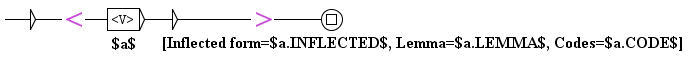
\includegraphics[width=16cm]{resources/img/fig6-17o.png}
\caption{Utilisation d'une variable de dictionnaire\label{fig-morpho5}}
\end{center}
\end{figure}

\begin{figure}[!ht]
\begin{center}
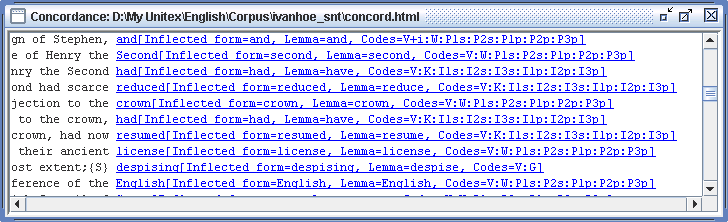
\includegraphics[width=15cm]{resources/img/fig6-17p.png}
\caption{Résultats de la  grammaire de la figure \ref{fig-morpho5} appliquée en mode in MERGE
\label{fig-morpho6}}
\end{center}
\end{figure}

\begin{figure}[!ht]
\begin{center}
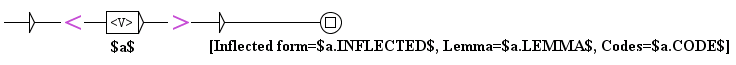
\includegraphics[width=15.5cm]{resources/img/fig6-17q.png}
\caption{Utilisation d'une variable de dictionnaire en mode normal\label{fig-morpho7}}
\end{center}
\end{figure}


\bigskip
\noindent \textbf{Variables de dictionnaire dans LocateTfst}

\noindent Pour les grammaires appliquées avec \verb+LocateTfst+ (cf. section~\ref{section-locate-tfst}), on dispose d'une possibilité
supplémentaire. 
En dehors du mode morphologique, on peut mémoriser dans une variable de dictionnaire
une étiquette lexicale contenue dans l'automate du texte.
Il suffit pour cela d'associer à la boîte une sortie de la forme \verb+$:abc$+ où \verb+abc+
est le nom de la variable.
On peut ensuite l'utiliser comme variable de dictionnaire habituelle, de la façon décrite ci-dessus~:
on peut obtenir la forme fléchie, la forme canonique et les codes donnés dans l'entrée, sa
catégorie grammaticale, ses codes sémantiques, ses codes flexionnels et la valeur
 \verb+zzz+ de l'attribut \verb+yyy+ s'il y figure un  code sémantique de la forme \verb+yyy=zzz+.


\section{Exploration des chemins d’une grammaire}
\index{Exploration des chemins d’une grammaire}

Il est possible de générer les chemins reconnus par une grammaire, par exemple pour
vérifier qu’elle engendre correctement les formes attendues. Pour cela, ouvrez le graphe
principal de votre grammaire et assurez-vous que la fenêtre du graphe est bien la fenêtre active
(la fenêtre active possède une barre de titre bleu, tandis que les fenêtres inactives ont une
barre de titre grise). Allez ensuite dans le menu "FSGraph", puis dans le sous-menu "Tools",
et cliquez sur "Explore graph paths". La fenêtre de la figure 
~\ref{fig-explore-graph-paths} apparaît alors.


\begin{figure}[!ht]
\begin{center}
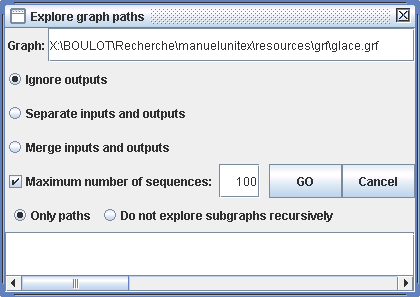
\includegraphics[width=10.4cm]{resources/img/fig6-18.png}
\caption{Exploration des chemins d’une grammaire\label{fig-explore-graph-paths}}
\end{center}
\end{figure}

\bigskip
\noindent Le cadre supérieur contient le nom du graphe principal de la grammaire à explorer.
Les options suivantes concernent la gestion des sorties de la grammaire ainsi que le mode
d’exploration:


\begin{itemize}
  \item "Ignore outputs": les sorties sont ignorées;
  \item "Separate inputs and outputs": les sorties sont affichées groupées après les entrées
  (\verb$ a b c / A B C$);
  \item "Merge inputs and outputs": chaque sortie est affichée immédiatement après l’entrée 
  	  qui lui correspond
  (\verb$a/A b/B c/C$).
  \item "Only paths": les appels aux sous-graphes sont explorés récursivement;
  \item "Do not explore subgraphs recursively": les appels aux sous-graphes sont affichés sans
être explorés récursivement.
\end{itemize}

\noindent Si l’option "Maximum number of sequences" est cochée, le nombre spécifié sera le nombre
maximum de chemins générés. Si l’option n’est pas sélectionnée, tous les chemins seront générés.


\bigskip
\noindent Voici ce que l’on obtient pour le graphe de la figure ~\ref{fig-glace} 
 avec les paramètres par défaut (ignorer les sorties, limite = 100 chemins) :


\bigskip
\noindent
\texttt{<NB> <boule> de glace \`a la pistache}

\noindent
\texttt{<NB> <boule> de glace \`a la fraise}

\noindent
\texttt{<NB> <boule> de glace \`a la vanille}

\noindent
\texttt{<NB> <boule> de glace vanille}

\noindent
\texttt{<NB> <boule> de glace fraise}

\noindent
\texttt{<NB> <boule> de glace pistache}

\noindent
\texttt{<NB> <boule> de pistache}

\noindent
\texttt{<NB> <boule> de fraise}

\noindent
\texttt{<NB> <boule> de vanille}

\noindent
\texttt{glace \`a la pistache}

\noindent
\texttt{glace \`a la fraise}

\noindent
\texttt{glace \`a la vanille}

\noindent
\texttt{glace vanille}

\noindent
\texttt{glace fraise}

\noindent
\texttt{glace pistache}

\begin{figure}[!ht]
\begin{center}
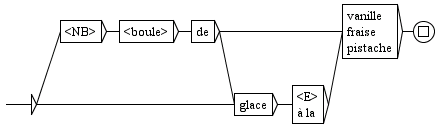
\includegraphics[width=10.9cm]{resources/img/fig6-19.png}
\caption{Exemple de graphe \label{fig-glace}}
\end{center}
\end{figure}




\section{Collection de graphes}
\index{Collection de graphes}

Il peut arriver que l’on souhaite appliquer plusieurs grammaires situées dans un même
répertoire. Pour cela, il est possible de construire automatiquement une grammaire à partir
d’une arborescence de fichiers. Supposons par exemple que l’on ait l’arborescence suivante:


\begin{itemize}
  \item \textit{Dicos}:
  \begin{itemize}
    \item \textit{Banque}:
    \begin{itemize}
      \item \texttt{carte.grf}
    \end{itemize}
    \item \textit{Nourriture}:
    \begin{itemize}
      \item \texttt{eau.grf}
      \item \texttt{pain.grf}
    \end{itemize}
    \item \texttt{truc.grf}
  \end{itemize}
\end{itemize}

\noindent Si l’on veut rassembler toutes ces grammaires en une seule, on peut le faire avec la
commande "Build Graph Collection" dans le sous-menu "FSGraph > Tools". On configure cette
opération au moyen de la fenêtre de la figure
~\ref{fig-build-graph-collection}.

\begin{figure}[!ht]
\begin{center}
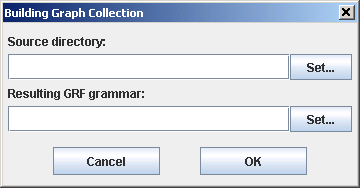
\includegraphics[width=9cm]{resources/img/fig6-20.png}
\caption{Construction d’une collection de graphes\label{fig-build-graph-collection}}
\end{center}
\end{figure}

\noindent Dans le champ "Source directory", sélectionnez le répertoire racine que vous voulez
explorer (dans notre exemple, le répertoire \textit{Dicos}).  Dans le champ "Resulting GRF grammar",
indiquez le nom de la grammaire produite.


\bigskip
\noindent ATTENTION : ne placez pas la grammaire de sortie dans l’arborescence que vous
voulez explorer, car dans ce cas, le programme va chercher à lire et à écrire simultanément
dans ce fichier, ce qui provoquera un plantage.


\bigskip
\noindent Lorsque vous cliquerez sur "OK", le programme recopiera les graphes dans le répertoire de
la grammaire de sortie, et créera des sous-graphes correspondant aux différents
sous-répertoires, comme on peut le voir sur la figure~\ref{fig-graph-collection}, qui montre
le graphe de sortie engendré pour notre exemple.


\bigskip
\noindent On peut constater qu’une boîte contient les appels à des
sous-graphes correspondant à des sous-répertoires (ici les répertoires \textit{Banque}
et \textit{Nourriture}), et que l’autre boîte fait appel à tous les graphes qui se trouvaient
dans le répertoire (ici le graphe \texttt{truc.grf}).

\begin{figure}[!ht]
\begin{center}
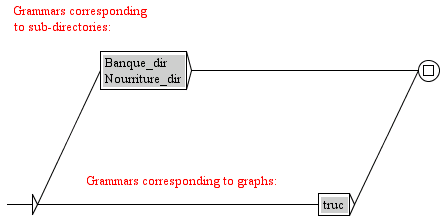
\includegraphics[width=11cm]{resources/img/fig6-21.png}
\caption{Graphe principal d’une collection de graphes\label{fig-graph-collection}}
\end{center}
\end{figure}



\section{Règles d’application des transducteurs}
\label{section-applying-transducers-rules}
\index{Transducteur!règles d'application}\index{Règles!pour l'application des transducteurs}
Cette section décrit les règles d’application des transducteurs lors des opérations de pré-
traitement et de recherche de motifs. Les graphes de flexion et de normalisation de formes
ambiguës ne sont pas concernés par ce qui suit.


\subsection{Insertion à gauche du motif reconnu}
\index{MERGE}\index{REPLACE}
Lorsqu’un transducteur est appliqué en mode REPLACE, les sorties remplacent les séquences lues dans le texte. 
%When a box in a transducer has no output, it is processed as if it had an \verb+<E>+ output.
En mode MERGE, les sorties sont insérées à gauche des séquences reconnues. Considérons le
transducteur de la figure~\ref{fig-transducer-example}
. 

\begin{figure}[!ht]
\begin{center}
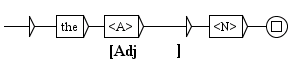
\includegraphics[width=7.2cm]{resources/img/fig6-22.png}
\caption{Exemple de transducteur\label{fig-transducer-example}}
\end{center}
\end{figure}

\bigskip
\noindent 
%Look at the transducer in Figure~\ref{fig-transducer-example}.
\noindent Si l’on applique ce transducteur au roman  \textit{Ivanhoe} by Sir Walter Scott
en mode MERGE, on obtient la concordance de la figure~\ref{fig-transducer-example-concordance} 


\begin{figure}[!ht]
\begin{center}
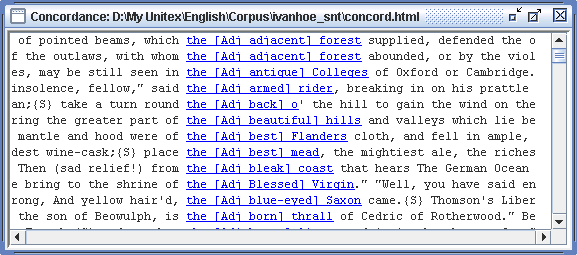
\includegraphics[width=14.4cm]{resources/img/fig6-23.png}
\caption{Concordance obtenue en mode MERGE avec le transducteur de la figure
~\ref{fig-transducer-example}\label{fig-transducer-example-concordance}}
\end{center}
\end{figure}

\subsection{Application en avançant}
Pendant les opérations de prétraitement, le texte est modifié au fur et à mesure qu’il
est parcouru. Afin d’éviter le risque de boucler indéfiniment, il ne faut pas que les 
séquences produites par un transducteur puissent être ré-analysées par celui-ci. Pour cette
raison, quand une séquence a été introduite dans le texte, l’application du transducteur se
poursuit après cette séquence.
Cette règle ne concerne que les transducteurs de prétraitement, car lors de l’application
de graphes syntaxiques, les sorties ne modifient pas le texte parcouru, mais un fichier de
concordances distinct du texte.


\subsection{Priorité à gauche}
\label{section-priorite-gauche}
\index{Priorité!à la séquence de gauche} \index{Chevauchement d'occurrences}
Lors de l’application d’une grammaire locale, les occurrences qui se chevauchent sont
toutes indexées.
Nous considérons, ici, de vrai chevauchements d'occurrence comme \verb+abc+ et \verb+bcd+, et
pas d'occurrences imbriquées comme \verb+abc+ et \verb+bc+.
Lors de la construction de la concordance, toutes ces occurrences sont présentées
(voir figure~\ref{fig-overlappping-occurrences}).

\begin{figure}[!ht]
\begin{center}
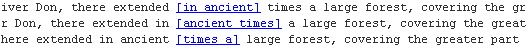
\includegraphics[width=13cm]{resources/img/fig6-24.png}
\caption{Occurrences se chevauchant dans une concordance\label{fig-overlappping-occurrences}}
\end{center}
\end{figure}

\noindent En revanche, si vous modifiez le texte au lieu de construire une concordance, il est
nécessaire de choisir parmi ces occurrences lesquelles seront prises en compte. Pour cela, Unitex
 applique la règle de priorité suivante : la séquence la plus à gauche l’emporte.

\bigskip
\noindent Si l’on applique cette règle aux trois occurrences de la concordance précédente, l’occurrence \textcolor{blue}{\texttt{[in ancient]}} est concurrente avec 
\textcolor{blue}{\texttt{[ancient times]}}. C’est donc la première qui
est retenue car c’est l’occurrence la plus à gauche, et \textcolor{blue}{\texttt{[ancient times]}} est
éliminée. L’occurrence suivante  \textcolor{blue}{\texttt{[times a]}} n’est donc plus en conflit avec 
\textcolor{blue}{\texttt{[ancient times]}} et peut donc apparaître dans le résultat:

\begin{center}
\texttt{...Don, there extended \textcolor{blue}{[in ancient] [times a]} large forest...}
\end{center}

\noindent La règle de priorité à gauche s’applique uniquement lorsque le texte est modifié, soit lors
du prétraitement, soit après l’application d’un graphe syntaxique (voir section 
~\ref{section-modifying-text}).

\subsection{Priorité aux séquences les plus longues}
\index{Priorité!à la séquence la plus longue}
Lors de l’application d’un graphe syntaxique, il est possible de choisir si la priorité doit
être donnée aux séquences les plus courtes ou les plus longues, ou si toutes les séquences
doivent être retenues. Lors des opérations de prétraitement, la priorité est toujours donnée
aux séquences les plus longues.


\subsection{Sorties à variables}
\label{section-variables}
\index{Variable!dans un graphe}\index{Sortie d'un transducteur!avec variable}
Comme nous l’avons vu à la section~\ref{section-using-variables}, il est possible d’utiliser
des variables d'entrée pour mémoriser le texte qui a été analysé par une grammaire. Ces variables
peuvent être utilisées dans les graphes de prétraitement et dans les graphes syntaxiques.

\bigskip
\noindent On doit donner des noms aux variables qu'on utilise. Ces noms peuvent contenir
les lettres comprises entre \verb+A+ et \verb+Z+, non accentuées minuscules ou majuscules, 
des chiffres et le caractère \verb+_+ (underscore).\index{Underscore}

\bigskip
\noindent Pour définir le début et la fin de la zone à stocker dans une variable d'entrée,
soit on utilise le bouton avec les parenthèses rouges dans la barre d'icônes au-dessus du graphe
(section ~\ref{toolbar-commands}),
soit on crée deux boîtes, l'une contenant le nom de la variable encadré par les caractères
\verb-$- et \verb-(- pour le début de la zone, et l'autre par \verb-$- et \verb-)- pour la fin.
Pour utiliser une variable dans une sortie, on fait précéder et suivre son nom du caractère \verb-$-
 (voir figure~\ref{fig-variable-definition}).

\bigskip
\noindent Les variables sont globales. Cela signifie qu'on peut définir une variable dans un
graphe et l’appeler dans un autre, comme l’illustrent les graphes de la figure
~\ref{fig-variable-definition}. Si on applique le graphe \verb+TitleName+ en mode MERGE au texte
\textit{Ivanhoe}, on obtient la concordance de la figure ~\ref{fig6-14}.

\bigskip
\noindent Les sorties à variables peuvent être utilisées pour déplacer des groupes de
mots.\index{Déplacement de groupes de mots} En effet,
l’application d’un transducteur en mode REPLACE n’écrit dans le texte que les séquences
produites par des sorties. Pour intervertir deux groupes de mots, il suffit donc de les stocker
dans des variables et de produire une sortie avec ces variables dans l’ordre souhaité. Ainsi,
le transducteur de la
figure~\ref{fig-swapping-words} appliqué en mode REPLACE au texte \textit{Ivanhoe}
donne la concordance de la figure~\ref{fig-no-space-problem}.

\begin{figure}[!htp]
\begin{center}
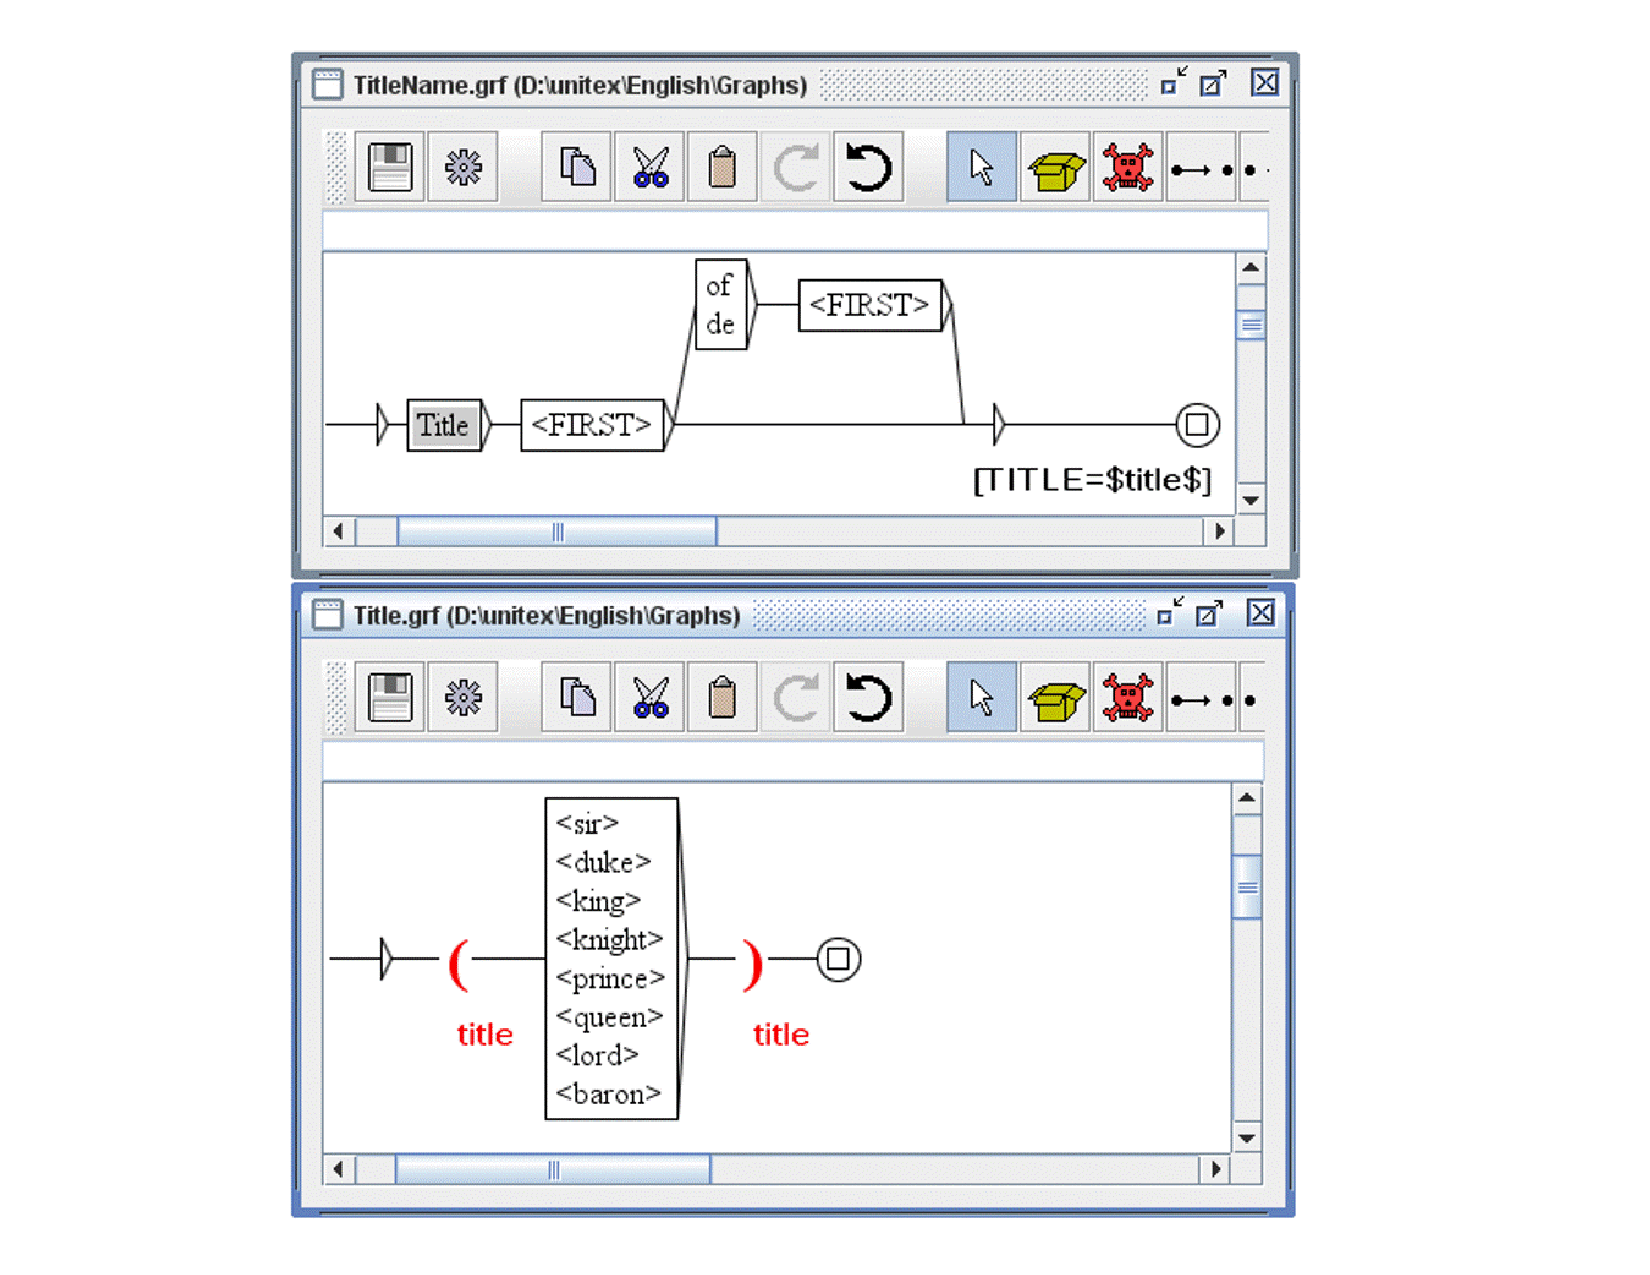
\includegraphics[width=16cm]{resources/img/fig6-25.pdf}
\caption{Définition d’une variable d'entrée dans un sous-graphe\label{fig-variable-definition}}
\end{center}
\end{figure}

\begin{figure}[!htp]
\begin{center}
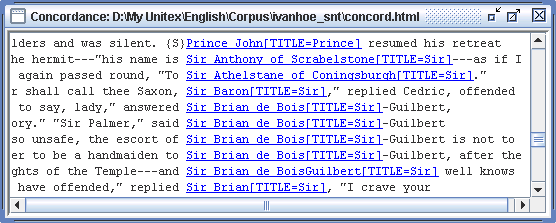
\includegraphics[width=13cm]{resources/img/fig6-26.png}
\caption{Concordance obtenue par l’application du graphe \texttt{TitleName}\label{fig6-14}
de la fig.~\ref{fig-variable-definition}
}
\end{center}
\end{figure}

\begin{figure}[!ht]
\begin{center}
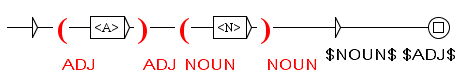
\includegraphics[width=11.3cm]{resources/img/fig6-27.png}
\caption{Interversion de mots grâce à deux variables d'entrée\label{fig-swapping-words}}
\end{center}
\end{figure}

\begin{figure}[!ht]
\begin{center}
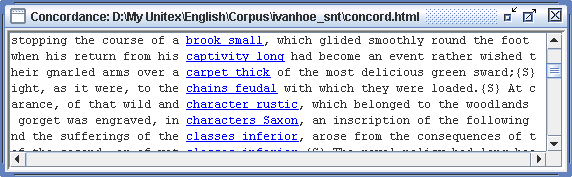
\includegraphics[width=13.4cm]{resources/img/fig6-28.png}
\caption{Résultat de l’application du transducteur de la figure~\ref{fig-swapping-words}\label{fig-no-space-problem}}
\end{center}
\end{figure}

\bigskip
\noindent Si le début ou la fin d’une variable est mal défini (fin d’une variable avant son début,
absence du début ou de la fin d’une variable), celle-ci sera ignorée lors des sorties.
Consultez la section \ref{section-advanced-search-options} pour d'autres options affectant
le traitement d'erreurs concernant les variables.

\bigskip
\noindent Il n’y a aucune limite au nombre de variables utilisables.

\bigskip
\noindent    Les variables d'entrées peuvent être imbriquées, et même se chevaucher comme le montre la
figure~\ref{fig-overlapping-variables}.

\begin{figure}[!ht]
\begin{center}
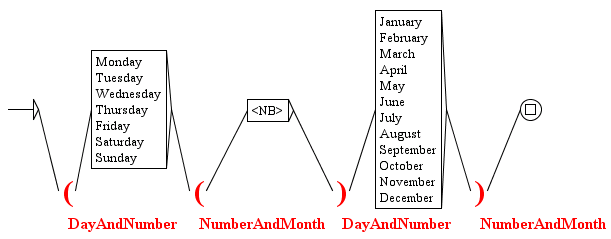
\includegraphics[width=15cm]{resources/img/fig6-29.png}
\caption{Chevauchement de variables d'entrée\label{fig-overlapping-variables}}
\end{center}
\end{figure}

%\clearpage


\newpage

\section{Variables de sortie}
\label{section-output-variables}
\index{Variable!de sortie}
Les variables d'entrée sont déclarées soit avec les parenthèses rouges de la barre d'icônes,
soit avec \verb+$xxx(+ et \verb+$xxx)+, et mémorisent des portions du
texte d'entrée. 
Il est aussi possible de mémoriser des parties des sorties produites par une grammaire.
Cela met en jeu des variables de sortie.
Ces variables sont déclarées soit avec l'icône des parenthèses bleues
dans la barre d'icônes au-dessus du graphe (section ~\ref{toolbar-commands}),
soit avec \verb+$|xxx(+ et \verb+$|xxx)+.
Elles apparaissent en bleu (voir figure~\ref{fig-output-variables}).
Cette grammaire appliquée en mode MERGE au texte \textit{Ivanhoe} produit la
concordance visible sur la figure~\ref{fig-output-variables-concord}. 

\begin{figure}[!ht]
\begin{center}
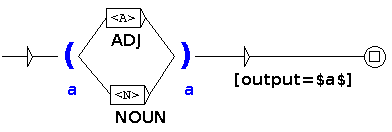
\includegraphics[width=8cm]{resources/img/fig6-17r.png}
\caption{Variables de sortie\label{fig-output-variables}}
\end{center}
\end{figure}

\begin{figure}[!ht]
\begin{center}
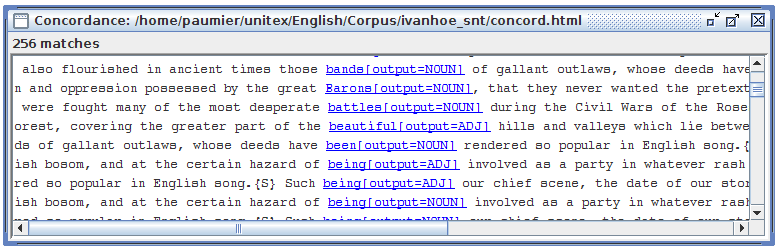
\includegraphics[width=15cm]{resources/img/fig6-17s.png}
\caption{Concordances obtenues avec la grammaire de la figure ~\ref{fig-output-variables}\label{fig-output-variables-concord}}
\end{center}
\end{figure}

\bigskip
\noindent Au moment où une variable de sortie est initialisée,
les séquences de sortie du transducteur ne sont pas émises dans la sortie correspondant à l'occurrence courante,
elles sont seulement mémorisées dans la variable de sortie créée par cette opération.
Par exemple, les sorties \verb+ADJ+ et \verb+NOUN+ de la figure figure~\ref{fig-output-variables}
n'ont pas été insérées à gauche du texte d'entrée
dans la figure~\ref{fig-output-variables-concord}.
Par ailleurs, les sorties sont traitées avant d'être mémorisées~: si la sortie d'une boite contient une chaine comme 
\verb+$A.LEMMA$+, la variable de sortie ne contiendra en fait pas cette chaîne mais le lemme associé à
la variable \verb+A+.

\bigskip
\noindent Les variables de sortie mémorisent seulement des sorties
effectivement produites par la grammaire. Ainsi, même en mode MERGE, les
variables de sortie ne mémorisent jamais le texte d'entrée
(figures~\ref{fig-output-variables} et \ref{fig-output-variables-concord}).

\bigskip
\noindent Quand une boite redéfinit une variable qui avait déjà été définie,
\index{Variable!redéfinition} la nouvelle valeur écrase l'ancienne.
Ainsi, si la variable est définie dans une boucle, la valeur de la variable juste après
la boucle dépend du dernier passage dans la boucle.


\section{Opérations sur les variables}
\label{section-ops-on-variables}
\subsection{Tests sur les variables}
\index{Tests sur les variables}\index{Variable!interrogation}

\noindent Il est possible de tester si une variable est définie ou non, afin d'interrompre la
reconnaissance courante si la condition n'est pas vérifiée. Ceci se fait en insérant la  séquence
\verb+$xxx.SET$+ dans la sortie d'une boîte. Ainsi, si une variable dénommée \verb+xxx+ a été définie,
cette séquence est ignorée et la reconnaissance continue, sinon, la reconnaissance s'arrête
et le programme repart en arrière. Ceci fonctionne sur les variables d'entrée, les variables de
sortie et les variables de dictionnaire. De façon similaire, on peut vérifier qu'une variable n'est
pas définie en utilisant \verb+$xxx.UNSET$+. La figure \ref{fig-testing-a-variable} montre un graphe
qui utilise ce type de test. La figure \ref{fig-testing-a-variable-results} montre les résultats obtenus par ce graphe en mode MERGE.

\begin{figure}[!ht]
\begin{center}
\includegraphics[width=9cm]{resources/img/fig6-29b.png}
\caption{Test d'une variable\label{fig-testing-a-variable}}
\end{center}
\end{figure}

\begin{figure}[!ht]
\begin{center}
\includegraphics[width=10cm]{resources/img/fig6-29c.png}
\caption{Résultats d'un test de variable\label{fig-testing-a-variable-results}}
\end{center}
\end{figure}


\subsection{Comparaison de variables}
\index{Comparaison!de variables}
Il est également possible de comparer tout type de variable (d'entrée, de sortie, ou de dictionnaire) avec une constante ou une autre variable. Ceci se fait en insérant dans la sortie d'une boîte une séquence respectant la syntaxe suivante~:


\bigskip
\noindent \verb+$abc.EQUAL=xyz$+

\bigskip
\noindent Cela agit comme un interrupteur qui permet de bloquer l'exploration de grammaire si la valeur de la variable \verb+abc+ est différente de la valeur de la variable \verb+xyz+. Remarquons que pour les variables de dictionnaire, c'est la forme fléchie telle qu'elle existe dans le dictionnaire (attention aux variantes de casse~!) qui est utilisée pour le test. Si vous désirez comparer la variable \verb+abc+ à la constante \verb+JKL+, utilisez le test suivant:

\bigskip
\noindent \verb+$abc.EQUAL=#JKL$+

\bigskip
\noindent on peut également tester si le contenu est différent avec \verb+UNEQUAL+.

\bigskip
\noindent Si vous désirez comparer des variables en ignorant les variantes de casse, vous pouvez
utiliser les tests suivants:

\bigskip
\noindent \verb+$abc.EQUALcC=xyz$+ \\
ou \\
\verb+$abc.UNEQUALcC=xyz$+

\subsection{Recherche d'un code sémantique dans une variable de dictionnaire}
\index{Variable!code sémantique}
On peut chercher dans une variable de dictionnaire \index{Variable!dictionary entry}
(section~\ref{dictionary-variables}) un ``code sémantique'' au sens de la section~\ref{section-DELAF-entry-syntax}.
Pour cela, on insère dans la sortie d'une boite une séquence respectant la syntaxe suivante~:

\bigskip
\noindent \verb+$abc.EQ=Conc$+

\bigskip
\noindent Ce test agit comme un interrupteur qui permet de bloquer l'exploration de la grammaire si \verb+Conc+
ne figure pas parmi les ``codes sémantiques'' de la variable de dictionnaire \verb+abc+. On peut chercher
un seul code à la fois dans une variable. Pour vérifier plusieurs codes, on met plusieurs boites en série.

\bigskip
\noindent Cette fonctionnalité est utilisée pour de grandes grammaires de graphes-dictionnaires morphologiques, en vue de
dissocier dans des boites distinctes la vérification d'un code grammatical et de ``codes sémantiques'' qui viennent ensuite,
comme dans \cite{paumier_nam_2014}, page~486.
On teste le code grammatical avec un masque lexical, puis on fait de même pour les codes sémantiques
en les cherchant dans la variable de dictionnaire correspondante.
Cette dissociation peut accélérer l'application des graphes si~:
\begin{itemize}
\item tous les graphes sont invoqués directement ou indirectement depuis un même graphe principal, 
\item le graphe principal est compilé et transformé en transducteur fini (voir section~\ref{flatten-section}),
\item la boite qui contient le masque lexical est commune à plus de chemins que celles qui cherchent les codes sémantiques
dans la variable de dictionnaire\footnote{De cette façon, le masque lexical provoque une consultation des dictionnaires du mode morphologique qui n'est effectuée qu'une fois avant plusieurs recherches de codes sémantiques.
Si on vérifie le code grammatical et un code sémantique par un même masque lexical, ces masques deviennent plus
nombreux dans l'ensemble de la grammaire et ils provoquent plus de consultations des dictionnaires.}.
\end{itemize}

\section{Application des graphes aux textes}
\label{section-applying-graphs-to-text}
Cette section concerne uniquement les graphes syntaxiques.
\subsection{Configuration de la recherche}
Pour appliquer un graphe à un texte, vous devez ouvrir le texte, puis cliquer sur "Locate
Pattern..." dans le menu "Text" ou appuyer sur <Ctrl+L>. Vous pouvez alors configurer votre
recherche grâce à la fenêtre de la figure
~\ref{fig-regexp-frame}.

\begin{figure}[!ht]
\begin{center}
\includegraphics[width=9cm]{resources/img/fig6-30.png}
\caption{Fenêtre de recherche d’expressions\label{fig-regexp-frame}}
\end{center}
\end{figure}

\index{Recherche de motifs}
\noindent Dans le cadre intitulé "Locate pattern in the form of", choisissez "Graph" et sélectionnez
votre graphe en cliquant sur le bouton "Set". Vous pouvez choisir un graphe au format
 \verb+.grf+ (Unicode Graphs) ou un graphe compilé au format \verb+.fst2+ format (Unicode
Compiled Graphs). Si votre graphe est au format \verb+.grf+, Unitex le compilera
 automatiquement avant de lancer la recherche. Si vous cliquez sur "Activate debug mode", la
 concordance sera affichée dans une fenêtre dans laquelle vous trouverez l'automate et, 
 pour chaque séquence reconnue, la liste des états du chemin qui la reconnaît. Cette fenêtre est décrite en détails à la section~\ref{section-debug-mode}.

\bigskip
\noindent Le cadre "Index" permet de sélectionner le mode de reconnaissance:

\index{Shortest matches}\index{Longest matches}\index{All matches}
\begin{itemize}
  \item "Shortest matches" : donne la priorité aux séquences les plus courtes;
  \item "Longest matches" :  donne la priorité aux séquences les plus longues. C’est le mode
utilisé par défaut;
  \item "All matches" : donne toutes les séquences reconnues.
\end{itemize}

\noindent 
Le cadre "Search limitation" permet de limiter ou non la recherche à un certain nombre
d’occurrences. Par défaut, la recherche est limitée aux 200 premières occurrences.
\index{Occurrences!nombre}

\bigskip
\index{MERGE}\index{REPLACE}
\noindent Le cadre "Grammar outputs" concerne le mode d’utilisation des sorties. Le mode "Merge
with input text" permet d’insérer les séquences produites par les sorties. Le mode "Replace
recognized sequences" permet de remplacer les séquences reconnues par les séquences produites.
Le troisième mode ignore les sorties. Ce dernier mode est utilisé par défaut.

\bigskip
\noindent
Dans le cadre "Search algorithm", vous pouvez spécifier si vous voulez effectuer la recherche sur le
texte en utilisant le programme Locate ou sur l'automate du texte avec LocateTfst.
Par défaut, la recherche est faite avec le programme Locate, comme Unitex l'a toujours fait jusqu'à
maintenant. Si vous désirez utiliser LocateTfst, lisez la section~\ref{section-locate-tfst}.

\bigskip
\noindent
Une fois vos paramètres fixés, cliquez sur "SEARCH" pour lancer la recherche.

%\clearpage

\subsection{Options de recherche avancées}
\index{Options de recherche avancées}
\label{section-advanced-search-options}
Si vous sélectionnez l'onglet "Advanced options", vous voyez le cadre de la
figure \ref{fig6-advanced-options1}.

\begin{figure}[!ht]
\begin{center}
\includegraphics[width=9cm]{resources/img/fig6-advanced-options1.png}
\caption{Options de recherche avancées\label{fig6-advanced-options1}}
\end{center}
\end{figure}

\bigskip
\index{Sortie d'un transducteur!ambiguïté}\index{Ambigu!transducteur}
\noindent L'option "Ambiguous output policy" est illustrée par le graphe de la 
figure \ref{fig6-advanced-options2}. Lorsqu'un déterminant est suivi par un mot pouvant être un
nom ou un adjectif, il peut produire deux sorties distinctes pour la même séquence d'entrée
(le transducteur est dit ambigu).

\bigskip
\begin{figure}[!ht]
\begin{center}
\includegraphics[width=9cm]{resources/img/fig6-advanced-options2.png}
\caption{Graphe avec des sorties ambiguës\label{fig6-advanced-options2}}
\end{center}
\end{figure}

\noindent Si nous appliquons ce graphe sur le texte \textit{Ivanhoe} avec l'option "Allow ambiguous outputs''
(celle par défaut), nous obtenons la concordance de la figure~\ref{fig6-advanced-options3}. Comme vous pouvez le constater, deux sorties sont produites pour la séquence \textit{the noble}.

\bigskip
\begin{figure}[!ht]
\begin{center}
\includegraphics[width=8.8cm]{resources/img/fig6-advanced-options3.png}
\caption{Sorties ambiguës pour \textit{the noble}\label{fig6-advanced-options3}}
\end{center}
\end{figure}

\noindent A l'opposé, avec l'option "Forbid ambiguous
outputs", nous obtenons la concordance de la figure \ref{fig6-advanced-options4},
avec seulement une sortie choisie arbitrairement pour la séquence \textit{the noble}.

\bigskip
\begin{figure}[!ht]
\begin{center}
\includegraphics[width=9cm]{resources/img/fig6-advanced-options4.png}
\caption{Sortie unique \textit{the noble}\label{fig6-advanced-options4}}
\end{center}
\end{figure}

\index{Traitement des erreurs sur les variables}
\bigskip
\noindent L'option "Variable error policy" permet de définir le comportement de
\verb+Locate+/\verb+LocateTfst+ lorsqu'ils rencontrent une sortie contenant une variable mal
définie. Remarquons que ce paramètre n'a aucun effet si les sorties sont ignorées. 
Considérons par exemple le graphe de la figure
\ref{fig6-advanced-options5}. 

\bigskip
\begin{figure}[!ht]
\begin{center}
\includegraphics[width=9cm]{resources/img/fig6-advanced-options5.png}
\caption{Une variable \textit{A} qui peut être indéfinie
\label{fig6-advanced-options5}}
\end{center}
\end{figure}

\noindent Avec l'option "Ignore variable errors", \textit{A} est ignorée, comme si son contenu était
vide, comme le montre la figure
\ref{fig6-advanced-options6}. 

\bigskip
\begin{figure}[!ht]
\begin{center}
\includegraphics[width=12cm]{resources/img/fig6-advanced-options6.png}
\caption{La variable \textit{A} peut être indéfinie
\label{fig6-advanced-options6}}
\end{center}
\end{figure}


\noindent Avec l'option "Exit on variable error", \verb+Locate+/\verb+LocateTfst+
émettent un message d'erreur, comme le montre la figure
\ref{fig6-advanced-options7}.

\bigskip
\begin{figure}[!ht]
\begin{center}
\includegraphics[width=9cm]{resources/img/fig6-advanced-options7.png}
\caption{Sortie à cause d'une variable erronée\label{fig6-advanced-options7}}
\end{center}
\end{figure}

\noindent Avec l'option "Backtrack on variable error" ,
\verb+Locate+/\verb+LocateTfst+ arrête l'exploration du chemin courant de la
grammaire. Ainsi, les variables jouent  le rôle d'interrupteurs qui coupent les chemins
lorsqu' elles sont indéfinies. Par exemple, l'application de la grammaire
\ref{fig6-advanced-options5} produit seulement des sorties contenant des adjectifs
, comme le montre la figure \ref{fig6-advanced-options8}. 

\bigskip
\begin{figure}[!ht]
\begin{center}
\includegraphics[width=13cm]{resources/img/fig6-advanced-options8.png}
\caption{Marche arrière en cas de variable erronée\label{fig6-advanced-options8}}
\end{center}
\end{figure}



\subsection{Concordance}
\index{Concordance}
Le résultat de la recherche est un fichier d’index contenant les positions de toutes les oc-
currences trouvées. La fenêtre de la figure~\ref{fig-configuration-display-occurrences}                                               vous propose de construire une concordance,
de modifier le texte ou de comparer le résultat de la recherche à la recherche précédente sur
le même texte.


\bigskip
\index{Contexte!concordance}\index{Tri!de concordance}
\noindent Pour afficher une concordance, vous devez cliquer sur le bouton "Build concordance".
Vous pouvez paramétrer la taille des contextes gauche et droit en caractères. Vous pouvez
également choisir le mode de tri qui sera appliqué aux lignes de la concordance grâce au
menu "Sort According to". Pour plus de détails sur les paramètres de construction de la
concordance, reportez-vous à la section~\ref{section-display-occurrences}.

\bigskip
\begin{figure}[!ht]
\begin{center}
\includegraphics[width=10cm]{resources/img/fig6-31.png}
\caption{Configuration de l’affichage des occurrences trouvées
\label{fig-configuration-display-occurrences}}
\end{center}
\end{figure}

\noindent La concordance est produite sous la forme d’un fichier HTML
\index{Fichier!HTML} Vous pouvez paramétrer Unitex pour que les concordances soient lues
à l’aide d’un navigateur Web (voir section~\ref{section-display-occurrences}).\index{Navigateur web}

\bigskip
\noindent Si vous affichez les concordances avec la fenêtre proposée par Unitex, vous pouvez accéder
à la séquence reconnue dans le texte en cliquant sur l’occurrence. Si la fenêtre du texte n’est pas
icônifiée et que le texte n’est pas trop long pour être affiché, vous verrez apparaître
la séquence sélectionnée (voir figure~\ref{fig-back-to-text}).

\bigskip
\begin{figure}[!ht]
\begin{center}
\includegraphics[width=13.5cm]{resources/img/fig6-32.png}
\caption{Sélection d’une occurrence dans le texte\label{fig-back-to-text}}
\end{center}
\end{figure}

\noindent De plus, si l’automate du texte a été construit et que la fenêtre correspondante n’est
pas icônifiée, le fait de cliquer sur une occurrence sélectionne l’automate de la phrase qui
contient cette occurrence.


\subsection{Modification du texte}
\label{section-modifying-text}
\index{Texte!modification}\index{Modification du texte}
Vous pouvez choisir de modifier le texte au lieu de construire une concordance. Pour
cela, sélectionnez un nom de fichier dans le cadre "Modify text" de la fenêtre de la figure
~\ref{fig-configuration-display-occurrences}. Ce fichier doit porter l’extension \verb+.txt+.
\index{Fichier!\verbc{.txt}}

\bigskip
\noindent Si vous souhaitez modifier le texte courant, il faut choisir le fichier \verb+.txt+                                                                                correspondant.
Si vous choisissez un autre nom de fichier, le texte courant ne sera pas affecté. Cliquez sur le
bouton "GO" pour lancer la modification du texte. Les règles de priorités appliquées lors de
cette opération sont détaillées à la section~\ref{section-applying-transducers-rules}.

\bigskip
\noindent Une fois cette opération effectuée, le fichier résultant est une copie du texte dans
laquelle les sorties ont été prises en compte. Les opérations de normalisation et de découpage en
unités lexicales sont automatiquement appliquées à ce fichier texte. Les dictionnaires du texte
existants ne sont pas modifiés. Ainsi, si vous avez choisi de modifier le texte courant, les 
modifications sont immédiatement effectives. Vous pouvez alors lancer de nouvelles recherches
sur le texte.


\bigskip
\noindent ATTENTION : si vous avez choisi d’appliquer votre graphe en ignorant les sorties, toutes
les occurrences seront effacées du texte.





\subsection{Extraction des occurrences}
\index{Extraction des occurrences}\index{Occurrences!extraction}
Vous pouvez extraire toutes les phrases du texte qui contiennent ou non des occurrences.
Pour cela, choisissez un nom de fichier de sortie grâce au bouton "Set File" dans le cadre
"Extract units" (figure~\ref{fig-configuration-display-occurrences}). Cliquez ensuite sur un des
boutons "Extract matching units" ou "Extract unmatching units" selon que vous voulez extraire les
phrases contenant les occurrences ou non.



\subsection{Comparaison de concordances}
\label{section-comparing-concordances}
\index{Comparaison!de concordances}\index{Concordance!comparaison}\index{Programmes
externes!\verbc{ConcorDiff}}
\index{\verbc{ConcorDiff}}
L’option "Show differences with previous concordance" permet de comparer la concordance
qui vient d’être calculée avec la concordance précédente, si elle existe. Pour cela, le programme
\verb+ConcorDiff+ construit les deux concordances dans l’ordre du texte, puis compare leurs lignes.
Le résultat est une page HTML qui montre alternativement les lignes des deux concordances, laissant
une ligne vide quand un match n'apparaît que dans une seule des deux concordances (figure~\ref{fig-concordiff}).

\begin{figure}[!ht]
\begin{center}
\includegraphics[height=10cm]{resources/img/fig6-33.png}
\caption{Exemple de comparaison de concordances\label{fig-concordiff}}
\end{center}
\end{figure}

\bigskip
\noindent Les lignes de la
concordance antérieure sont grisées et celles de la concordance courante restent sur fond blanc.
Dans chaque ligne, seules les séquences reconnues sont colorées. On peut cliquer dessus pour
ouvrir le texte à cette position.

\bigskip
\noindent Le bleu indique qu'une séquence est commune aux deux concordances. Le rouge indique qu'une séquence
reconnue est commune aux deux concordances, mais avec des extensions différentes, c'est-à-dire que les
deux séquences reconnues se chevauchent partiellement. Le vert signale qu'une séquence n'apparait
que dans une seule concordance.

\bigskip
\noindent S'il n'existe pas de concordance antérieure, le bouton est désactivé.

%\clearpage
\subsection{Mode Debug}
\label{section-debug-mode}
Lorsqu'on applique un graphe à un texte avec le menu \verb+Locate+ dans la fenêtre de la
figure~\ref{fig-regexp-frame}, si le mode debug est activé dans le champ "Locate pattern in the
form of", la concordance est affichée dans une fenêtre spéciale (voir figure~\ref{fig-debug-mode}),
divisée en trois parties~:

\begin{figure}[!ht]
\begin{center}
\includegraphics[height=9.5cm]{resources/img/fig6-34.png}
\caption{La fenêtre de concordance en mode debug\label{fig-debug-mode}}
\end{center}
\end{figure}

\medskip 
\indent En haut à droite, se trouve la fenêtre de concordance. Elle est identique à la fenêtre habituelle dans laquelle les séquences reconnues apparaissent en bleu.

\medskip
\indent En bas à droite se trouve le graphe utilisé par \verb+Locate+.

\medskip
\indent A gauche, il y a un tableau divisé en trois colonnes: "Tag", "Output" et "Matched".
Chaque token de la séquence reconnue apparaît dans la colonne "Matched", la colonne "Tag" indique le
contenu de la boîte de l'automate qui l'a reconnue, et si elle possède une sortie, elle apparaît
dans la colonne "Output".

\bigskip
\noindent Pour chaque séquence reconnue de la concordance, si on clique dessus, le tableau est
mis à jour. Si on clique sur une ligne du tableau, le système colore la boîte correspondante dans le graphe.
On peut ainsi voir pour chaque occurrence reconnue dans le texte quel chemin de l'automate la
reconnait. Le nombre en rouge au-dessus d'une boîte indique le nombre de  séquences du texte
pour lesquelles cette boîte a reconnu un token.

\bigskip
\noindent Quand on applique un graphe en mode debug avec le menu \verb+Text>Locate Pattern+,
le système le compile en un fichier \verb+fst2+ dans un formal spécial de mode debug, qui n'est
pas compatible avec CasSys. Voir la section~\ref{graphs-for-cassys} pour résoudre ce problème.
